% =====================================================================
%  Shared control for a brain-controlled wheelchair -- main report
%  Pragyan Mohanty, roll 24250
%
%  Compile from this folder (report/):
%      pdflatex report.tex
%      pdflatex report.tex      (second run fixes cross-references)
%  Figures are read straight from ../results/.
% =====================================================================
\documentclass[11pt,a4paper]{article}

\usepackage[T1]{fontenc}
\usepackage[utf8]{inputenc}
\usepackage{lmodern}
\usepackage{microtype}
\usepackage[margin=2.2cm]{geometry}
\usepackage{amsmath,amssymb}
\usepackage{graphicx}
\usepackage{booktabs}
\usepackage{array}
\usepackage{caption}
\usepackage{float}
\usepackage{xcolor}
\usepackage{tikz}
\usetikzlibrary{arrows.meta}
\usepackage[colorlinks=true,linkcolor=black,citecolor=black,urlcolor=blue]{hyperref}

\graphicspath{{../results/part1/figures/}{../results/part2/figures/}}

\captionsetup{font=small,labelfont=bf,justification=raggedright,singlelinecheck=true}
\setlength{\parindent}{0pt}
\setlength{\parskip}{0.5em}
\setlength{\emergencystretch}{2em}
\renewcommand{\topfraction}{0.9}
\renewcommand{\bottomfraction}{0.8}
\renewcommand{\textfraction}{0.07}
\renewcommand{\floatpagefraction}{0.8}
\setcounter{topnumber}{3}
\setcounter{totalnumber}{4}

% Pointers to the notebooks: [P2 §6.9] = Section 6.9 of
% src/part2_shared_control.ipynb.
\newcommand{\ptwo}[1]{{\small\textsf{[P2~\S#1]}}}
\newcommand{\pone}[1]{{\small\textsf{[P1: #1]}}}
\newcommand{\code}[1]{\texttt{#1}}
\newcommand{\uu}{u_{\mathrm{user}}}
\newcommand{\ua}{u_{\mathrm{auto}}}
\newcommand{\TTC}{\mathrm{TTC}}

\begin{document}

% ---------------------------------------------------------------------
\begin{center}
{\LARGE\bfseries Shared Control for a Brain-Controlled Wheelchair}\\[0.5em]
{\large How much control should an unreliable EEG decoder get?}\\[0.9em]
Pragyan Mohanty \quad (Roll No.\ 24250)\\[0.2em]
Control Systems course project
\end{center}

\begin{abstract}
\noindent
A brain--computer interface (BCI) can let a person steer a wheelchair by
imagining movements: imagining the left hand turns left, the right hand
turns right, the feet move forward and the tongue stops. The EEG decoder
behind such an interface is unreliable. On the nine subjects of BCI
Competition IV dataset 2a, our decoder (Common Spatial Patterns + Linear
Discriminant Analysis, with calibrated probabilities; trained on day~1,
tested on day~2) is right only \textbf{44\%} of the time (chance is
25\%), needs \textbf{2--4\,s} to decide, and on about half of all trials
never becomes confident. A simulated wheelchair driven by this decoder
alone reaches its goal in only \textbf{12\%} of drives.

Instead of trying to build a better decoder, we treat it as a fixed,
imperfect sensor and ask a control question: \emph{how should control be
shared between the user and an autopilot?} The motors receive
$u = \alpha\,\uu + (1-\alpha)\,\ua$, where $\alpha$ is the user's share.
We built a closed-loop simulator in which the user's commands pass
through a model of the real decoder (its errors, delays and confidence,
measured subject by subject), and compared six rules for choosing
$\alpha$ over 32,400 simulated drives in three rooms.

The best rule gives the user control in proportion to the decoder's
confidence $c$ and takes it away as the risk $r$ of a collision rises:
$\alpha = c\,(1-r)$, with risk computed from the time to collision. It
reaches the goal in \textbf{99.6\%} of drives, gives the user about 12\%
of the control on average, and works for every subject, including one
whose decoder is worse than chance. It is as safe as the autopilot alone
but not better, and switching parts off shows that the \emph{risk} term,
not the confidence, does the work. On the control-theory side we derive
exactly the largest loop delay the shared loop can tolerate,
$\tau_{\max}(\alpha)$: 0.529\,s when the user drives alone, and no limit
at all when the user's share is below 0.44. Direct simulation confirms
the formula. The overall conclusion is that this system is limited by
the decoder's \emph{errors}, not by its delay.
\end{abstract}

\paragraph{About this report.} This report presents the problem, the
method and the results. The full theory is also written in the two
notebooks in \code{src/}, alongside the code, and the step-by-step
stability derivation is in \code{report/math\_derivation.pdf}.

% =====================================================================
\section{Introduction}

\subsection{The problem}
A motor-imagery BCI reads EEG from the scalp while the user imagines a
movement, and turns each imagined movement into a command. For a
wheelchair, this command channel has three weaknesses:
\begin{itemize}\setlength{\itemsep}{1pt}
\item it is often \textbf{wrong} (our decoder: 56\% of decisions on
average);
\item it is \textbf{late} (2--4\,s to reach a confident decision);
\item it is \textbf{slow} (one new decision every 2\,s).
\end{itemize}
A wheelchair that obeys such a channel directly crashes most of the
time. The usual response is to improve the decoder. Here the decoder is
kept as it is, and the question becomes one for the controller.

\subsection{The idea}
Give the wheelchair a second driver, an autopilot that sees the room and
the goal, and mix the two commands:
\begin{equation}
\boxed{\;u = \alpha\,\uu + (1-\alpha)\,\ua, \qquad \alpha \in [0,1]\;}
\label{eq:blend}
\end{equation}
$\alpha = 1$ means the user drives alone and $\alpha = 0$ means the
autopilot drives alone. Mixing a human command with an autonomous one is
a standard form of \emph{shared control}~\cite{dragan2013blending}, and
has been used for brain-controlled wheelchairs~\cite{carlson2013wheelchairs}.
The question is \emph{how to choose $\alpha$}. The rule we propose uses
two signals:
\begin{equation}
\boxed{\;\alpha = c\,(1 - r)\;}
\label{eq:adaptive-short}
\end{equation}
where $c \in [0,1]$ is the decoder's confidence (``is this what the user
meant?'') and $r \in [0,1]$ is the risk of obeying the user's command
(``does it matter if it is wrong?''), computed from the time to
collision. The full rule (Section~\ref{sec:rules}) adds a switch and
smoothing so that $\alpha$ does not jump.

\subsection{What I did}
\begin{enumerate}\setlength{\itemsep}{1pt}
\item \textbf{Built and measured an EEG decoder} on a public dataset
(Part~1): accuracy, calibration of its confidence, confusion between
classes, and decision latency, for each of 9 subjects.
\item \textbf{Turned those measurements into a command-channel model}
that reproduces each subject's errors, delays and confidence.
\item \textbf{Built a closed-loop wheelchair simulator} with a user
model, an autopilot, a risk signal, and six rules for sharing control
(Part~2), and compared the rules over 32,400 paired drives.
\item \textbf{Derived the stability boundary} $\tau_{\max}(\alpha)$ of the
shared loop under delay exactly, and checked it by direct simulation.
\end{enumerate}

% =====================================================================
\section{The dataset}
\label{sec:data}

\subsection{BCI Competition IV, dataset 2a}
We use the public \emph{BCI Competition IV dataset 2a}, recorded at Graz
University of Technology~\cite{brunner2008graz,tangermann2012review}.
It is also distributed as \code{BNCI2014\_001}, which is the name used
by the MOABB library~\cite{jayaram2018moabb} that loads it in our code.

\begin{table}[H]
\centering\small
\begin{tabular}{@{}ll@{}}
\toprule
Subjects & 9 healthy subjects \\
Task & cue-based motor imagery, 4 classes: left hand, right hand, both feet, tongue \\
Sessions & 2 per subject, recorded on different days \\
Trials & 6 runs $\times$ 48 trials = 288 per session (72 per class) \\
Channels & 22 EEG electrodes (plus 3 EOG channels, which we drop) \\
Sampling & 250\,Hz, band-pass 0.5--100\,Hz, 50\,Hz notch filter \\
\bottomrule
\end{tabular}
\caption{Summary of the dataset.}
\label{tab:dataset}
\end{table}

\textbf{One trial.} At $t = 0$ a fixation cross appears on the screen. At
$t = 2$\,s an arrow (left, right, down or up) cues one of the four
classes, and the subject imagines that movement until about $t = 6$\,s.
We use the window from 0.5\,s to 2.5\,s after the cue, where the imagery
is under way.

\textbf{How we use the two days.} The decoder is trained only on day~1
and tested only on day~2. This is harder than testing on the same day,
because EEG changes between sessions, but it is what a real user would
face: a decoder trained yesterday, used today.

\textbf{Links.}
\begin{itemize}\setlength{\itemsep}{1pt}
\item Dataset description (PDF):
\url{https://www.bbci.de/competition/iv/desc_2a.pdf}
\item Competition page: \url{https://www.bbci.de/competition/iv/}
\item Download: the Part~1 notebook downloads it automatically through
MOABB (about 750\,MB, into \code{\textasciitilde/mne\_data});
documentation:
\url{https://neurotechx.github.io/moabb/generated/moabb.datasets.BNCI2014_001.html}
\end{itemize}

\subsection{From imagined movement to wheelchair command}
Each class is mapped to a wheelchair command relative to the direction
the chair is facing \ptwo{2.3}:

\begin{table}[H]
\centering\small
\begin{tabular}{@{}lll@{}}
\toprule
Imagined movement & Wheelchair command & Direction \\
\midrule
left hand  & turn left  & $+90^\circ$ \\
right hand & turn right & $-90^\circ$ \\
both feet  & move forward & $0^\circ$ \\
tongue     & stop       & --- \\
\bottomrule
\end{tabular}
\caption{Class-to-command mapping.}
\label{tab:mapping}
\end{table}

\begin{figure}[htbp]
\centering
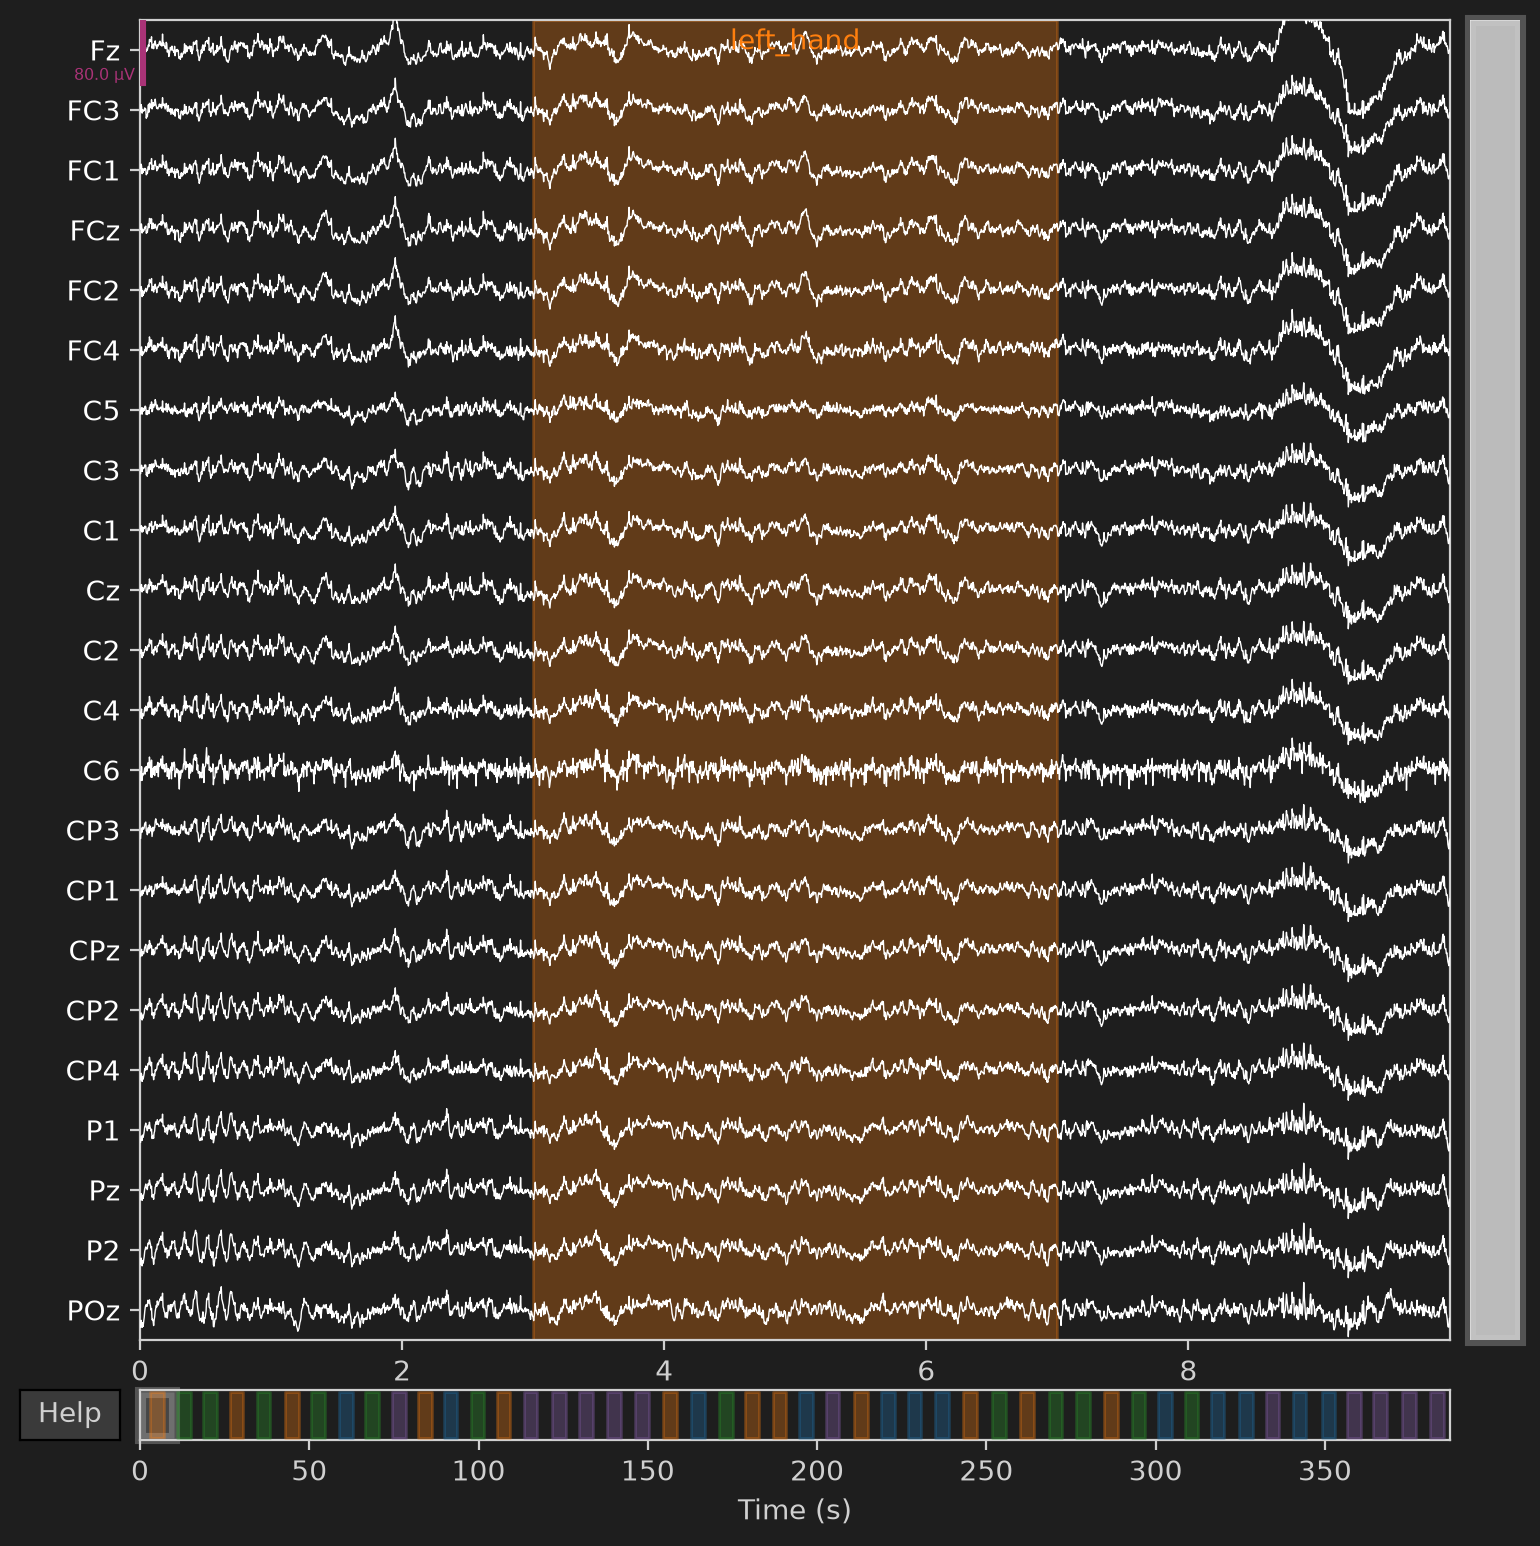
\includegraphics[width=0.5\textwidth]{raw_eeg.png}
\caption{Raw EEG of subject 3, all 22 channels, first 10\,s of a run.
The shaded block is one cued trial (left hand). The imagined movement is
not visible by eye; it shows up only as small power changes in the
8--30\,Hz band, which is why a decoder is needed \pone{Visualise the data}.}
\label{fig:raweeg}
\end{figure}

% =====================================================================
\section{Part 1: the EEG decoder}

\subsection{Method}
The pipeline has four steps \pone{Run all 9 subjects}, code in
\code{src/decoder/}:
\begin{enumerate}\setlength{\itemsep}{2pt}
\item \textbf{Band-pass filter} each channel to 8--30\,Hz (4th-order
Butterworth). Imagined movement changes the power of the $\mu$
(8--12\,Hz) and $\beta$ (13--30\,Hz) rhythms over the motor cortex.
\item \textbf{Common Spatial Patterns (CSP)}~\cite{ramoser2000csp}. For
two classes with average channel covariance matrices $\Sigma_1$ and
$\Sigma_2$, CSP finds spatial filters $w$ (weights over the 22 channels)
that maximise the variance of one class relative to the other:
\begin{equation}
w^{*} = \arg\max_{w}\; \frac{w^{\!\top}\Sigma_1 w}{w^{\!\top}\Sigma_2 w}.
\end{equation}
The solutions are generalised eigenvectors of $(\Sigma_1, \Sigma_2)$.
We use 6 filters (MNE's multi-class version), and the feature of each
filter is the logarithm of the filtered signal's variance.
\item \textbf{Linear Discriminant Analysis (LDA)} with shrinkage of the
covariance estimate~\cite{blankertz2011shrinkage} classifies the 6
features into one of the 4 classes, giving a probability for each.
\item \textbf{Platt calibration}~\cite{platt1999sigmoid}. LDA's
probabilities are often over- or under-confident. Day~1 is split 75/25;
the decoder is fitted on 75\% and a sigmoid is fitted on the other 25\%
to rescale its scores, so that a stated confidence of 70\% means the
decoder is right about 70\% of the time.
\end{enumerate}

\textbf{Metrics.} \emph{Accuracy} is the share of day-2 trials classified
correctly. \emph{Cohen's $\kappa$} corrects it for chance,
$\kappa = (p_o - p_e)/(1 - p_e)$, with $p_e = 0.25$ here. The
\emph{expected calibration error} groups trials into 10 confidence bins
$B_m$ and averages the gap between confidence and accuracy:
\begin{equation}
\mathrm{ECE} = \sum_{m=1}^{10} \frac{|B_m|}{n}\,
\bigl|\,\mathrm{acc}(B_m) - \mathrm{conf}(B_m)\,\bigr| .
\end{equation}
\emph{Decision latency}: the 2\,s window is slid forward in 0.1\,s steps,
and the latency is the end of the first window whose calibrated
confidence passes 0.5. Trials that never pass are \emph{censored} at
4\,s rather than dropped, since dropping them would hide exactly the
trials where the decoder is unsure.

\subsection{Results}

\begin{table}[H]
\centering\small
\begin{tabular}{@{}crrrrrrr@{}}
\toprule
 & & & \multicolumn{3}{c}{ECE (lower is better)} & Median & Never \\
\cmidrule(lr){4-6}
Subject & Accuracy & $\kappa$ & calibrated & raw$^{a}$ & raw$^{b}$ & latency (s) & confident \\
\midrule
1 & 0.556 & 0.407 & 0.150 & 0.138 & 0.158 & 2.00 & 0.12 \\
2 & 0.556 & 0.407 & 0.075 & 0.150 & 0.167 & 3.55 & 0.46 \\
3 & 0.691 & 0.588 & 0.044 & 0.146 & 0.164 & 2.00 & 0.02 \\
4 & 0.389 & 0.185 & 0.077 & 0.142 & 0.131 & 4.00 & 1.00 \\
5 & 0.191 & $-$0.079 & 0.144 & 0.148 & 0.268 & 4.00 & 0.92 \\
6 & 0.379 & 0.171 & 0.030 & 0.188 & 0.190 & 4.00 & 0.83 \\
7 & 0.396 & 0.194 & 0.188 & 0.299 & 0.371 & 2.00 & 0.02 \\
8 & 0.496 & 0.329 & 0.094 & 0.091 & 0.122 & 3.70 & 0.40 \\
9 & 0.337 & 0.116 & 0.063 & 0.157 & 0.192 & 4.00 & 0.99 \\
\midrule
\textbf{Mean} & \textbf{0.443} & \textbf{0.258} & \textbf{0.096} & \textbf{0.162} & \textbf{0.196} & --- & 0.53 \\
\bottomrule
\end{tabular}
\caption{Decoder results on day 2 (chance accuracy is 0.25). Raw ECE is
the calibration error before Platt scaling, scored in two ways:
$^{a}$against the raw prediction (as in \code{summary\_by\_subject.csv}
and Figure~\ref{fig:calib}); $^{b}$against the calibrated prediction,
which is the decision the wheelchair actually uses. ``Never confident'' is
the share of trials that never reached 50\% confidence within 4\,s.}
\label{tab:decoder}
\end{table}

\textbf{Accuracy.} The mean accuracy is \textbf{0.443}: well above chance,
but wrong more often than right. It varies widely, from 0.691
(subject~3) to 0.191 (subject~5). Subject~5 is \emph{below} chance
($\kappa = -0.079$); we keep this subject on purpose, because a bad
decoder is exactly where shared control has to prove itself.

\textbf{Calibration.} Platt scaling lowers the mean ECE from 0.162 to
\textbf{0.096} and helps most subjects (Figure~\ref{fig:calib}).

\begin{figure}[htbp]
\centering
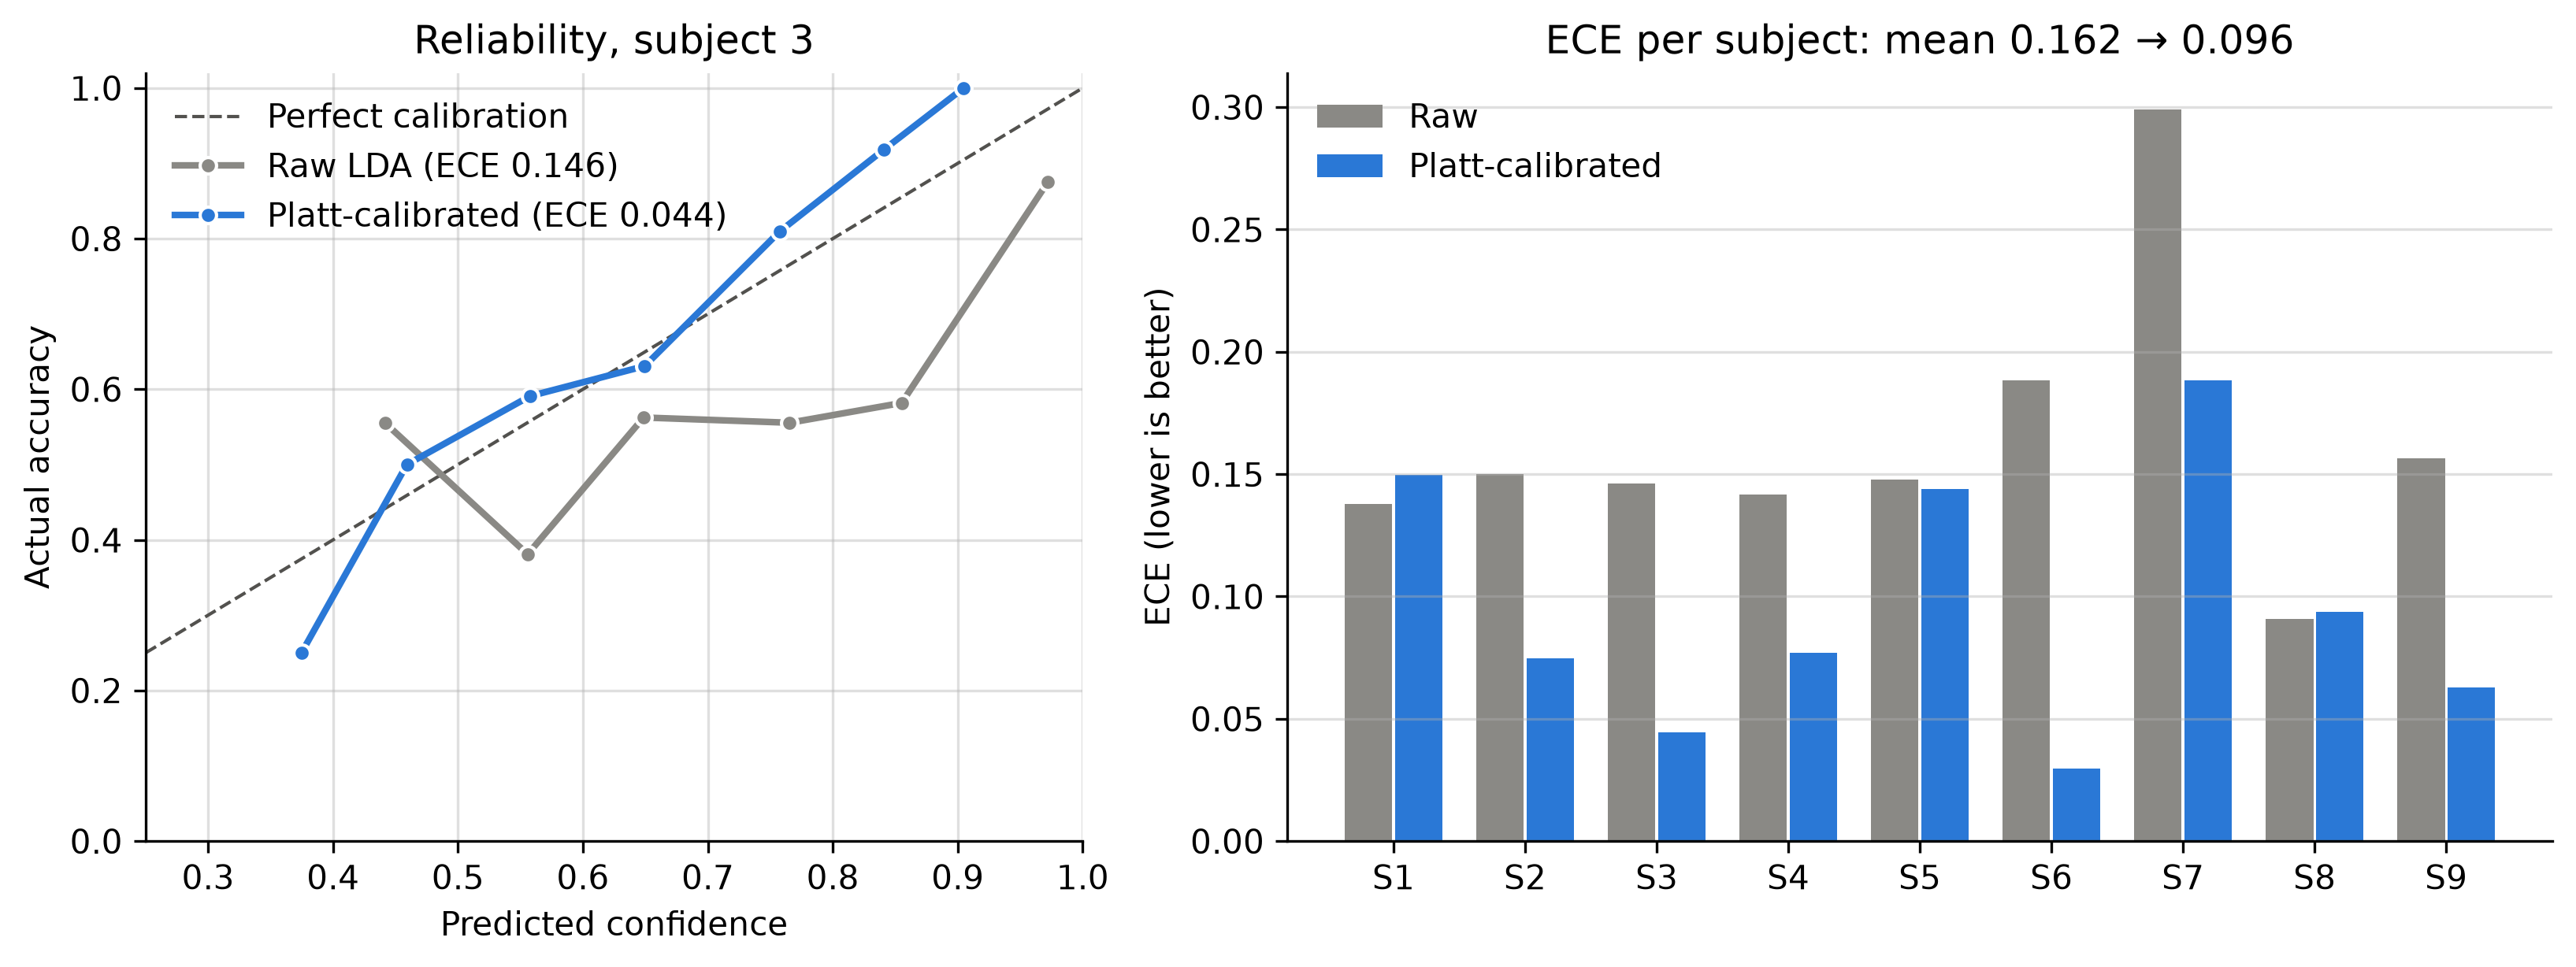
\includegraphics[width=0.85\textwidth]{fig2_calibration.png}
\caption{Calibration. Left: for subject 3, the calibrated confidence
follows the real accuracy (dashed diagonal) much more closely than the
raw LDA output. Right: ECE per subject before and after calibration.}
\label{fig:calib}
\end{figure}

\textbf{Where the errors go.} The confusion matrices
(Figure~\ref{fig:confusion}) show that errors are not spread evenly. They
depend strongly on \emph{which class was cued}: subject~1, for example,
is wrong on 85\% of \emph{feet} trials but on only 7\% of \emph{tongue}
trials, and when it misreads \emph{feet} (forward) it usually outputs
\emph{tongue} (stop). This matters for the wheelchair, because the
\emph{kind} of wrong command decides how dangerous an error is, and it
is why Part~2 draws each wrong command from the subject's own confusion
matrix rather than at random.

\begin{figure}[htbp]
\centering
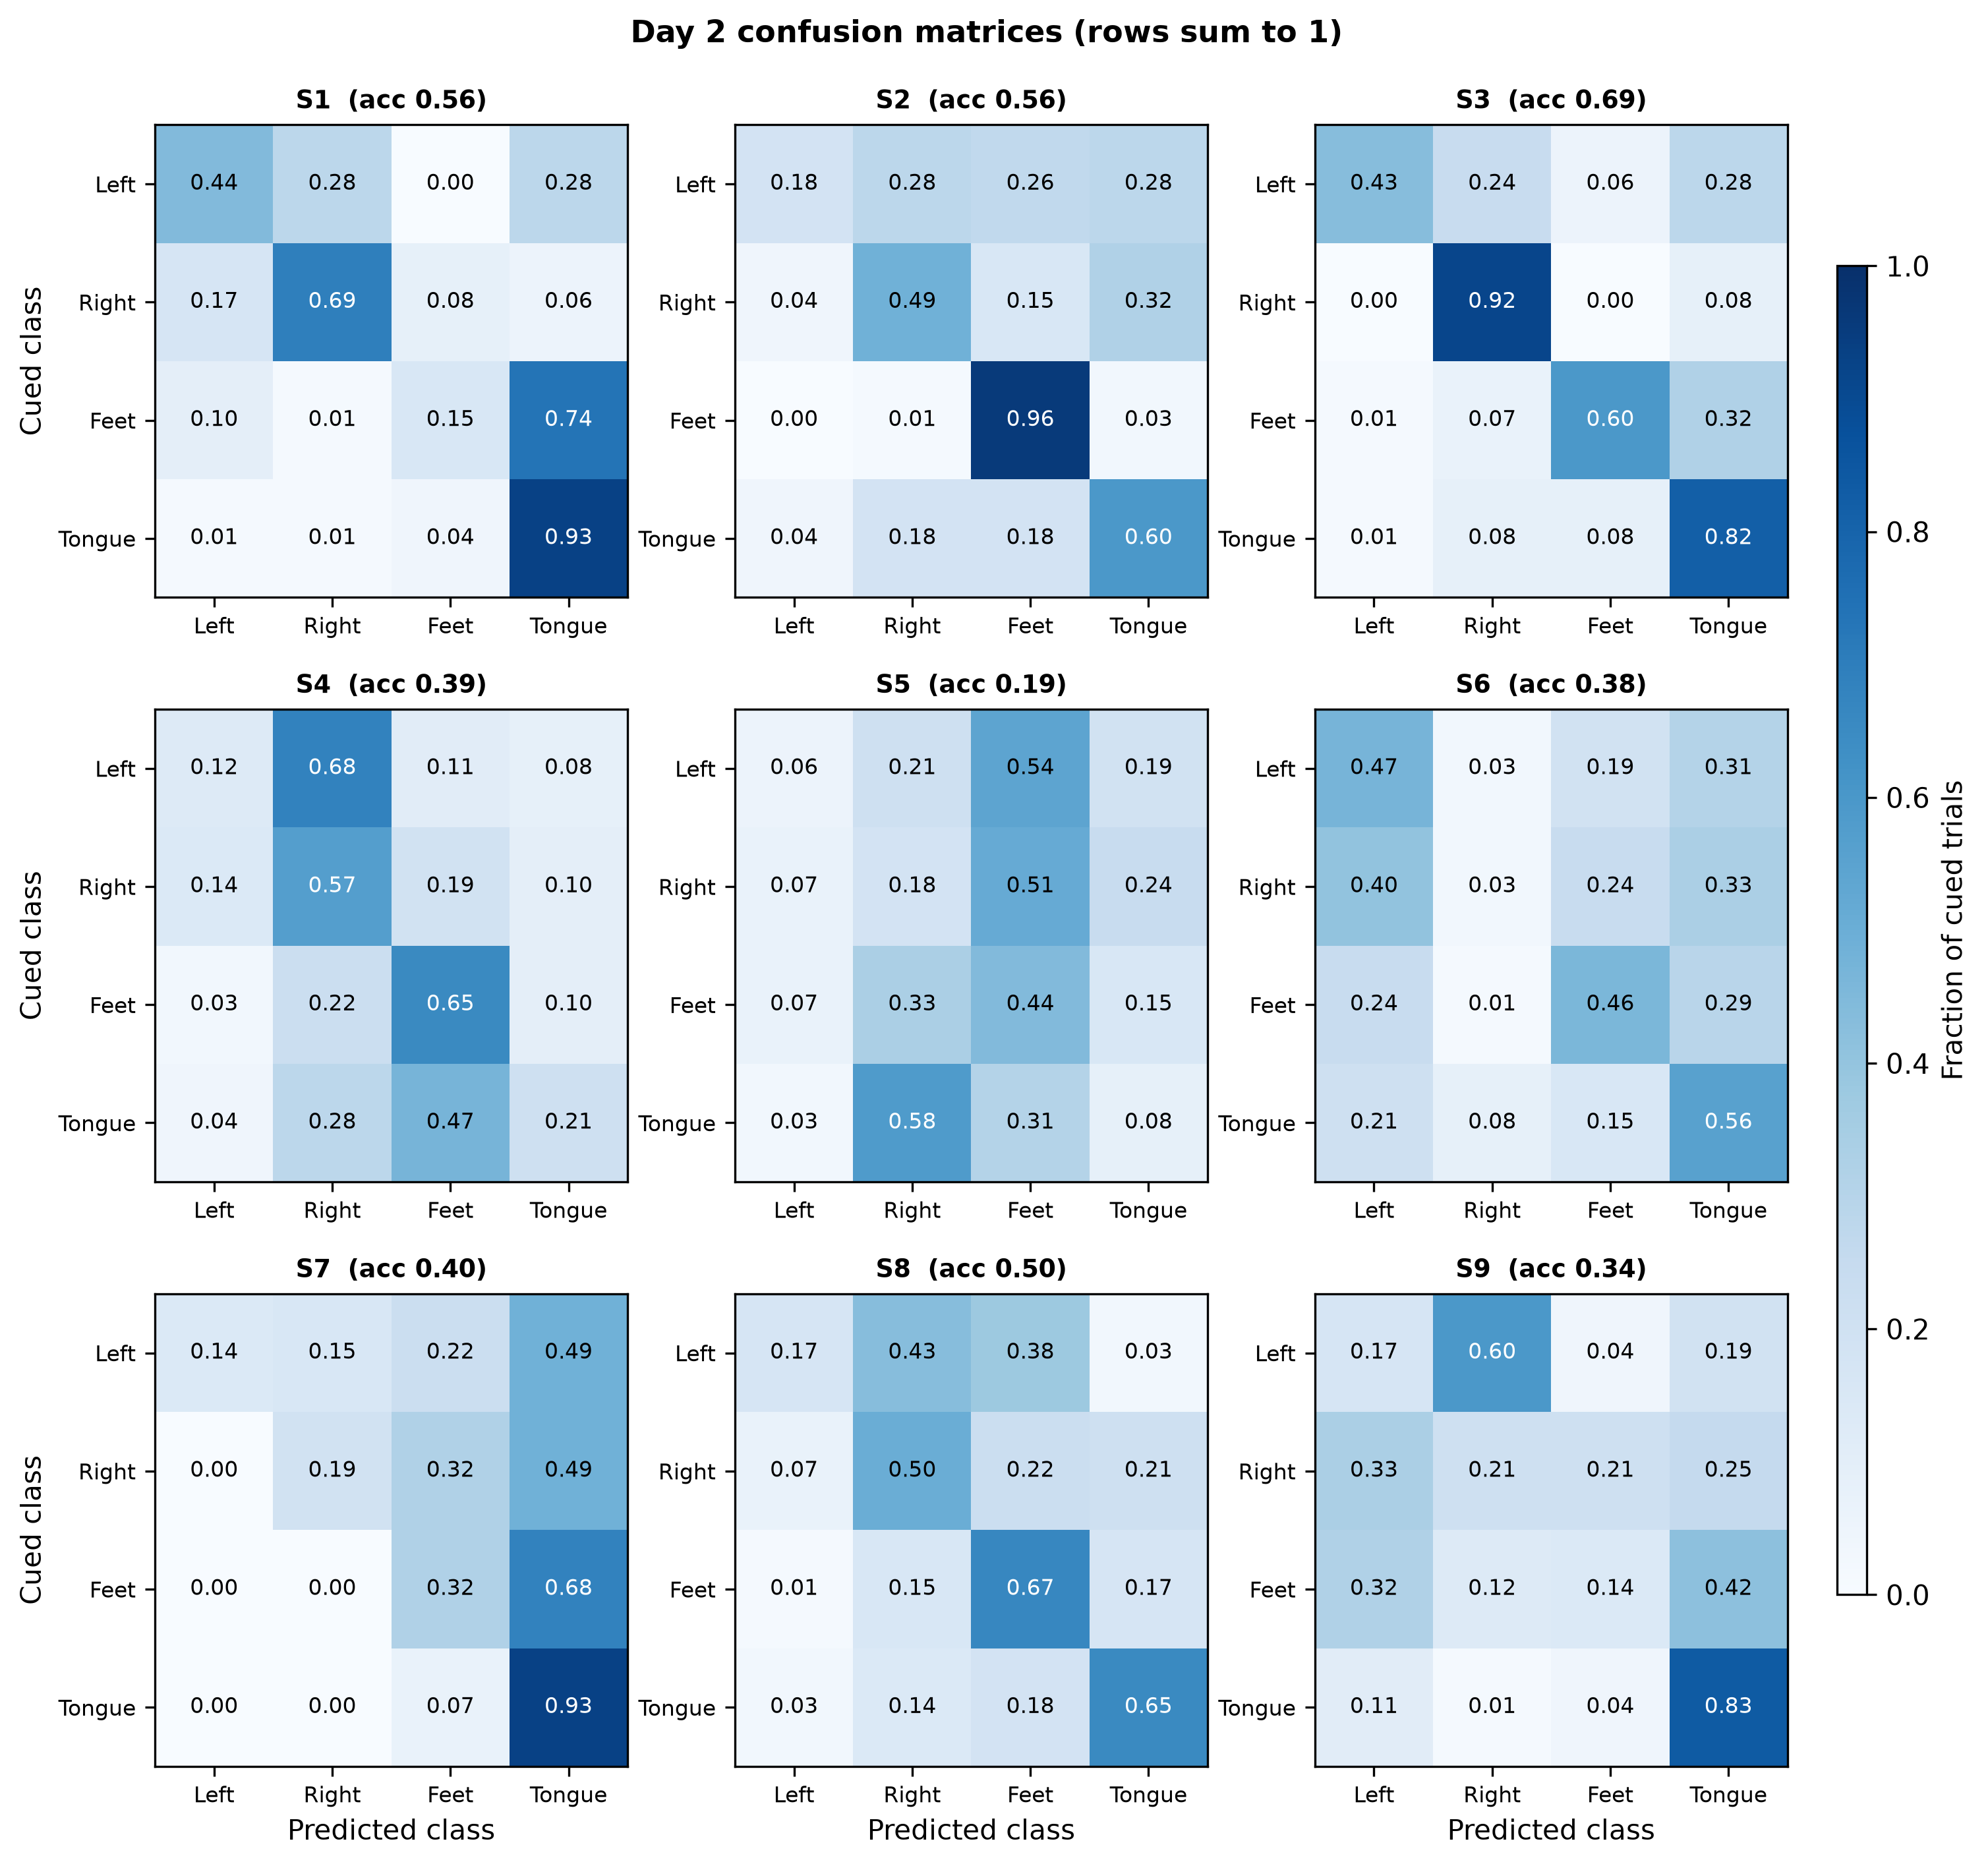
\includegraphics[width=0.6\textwidth]{fig3_confusion_matrices.png}
\caption{Day-2 confusion matrices for all 9 subjects (rows: cued class;
columns: decoded class).}
\label{fig:confusion}
\end{figure}

\textbf{What the decoder learned.} The CSP patterns of subject~3
(Figure~\ref{fig:csp}) sit over the motor cortex (around electrodes C3,
Cz and C4), which is where imagined hand and foot movement is expected.
This is a sanity check that the decoder uses brain activity and not
noise.

\begin{figure}[htbp]
\centering
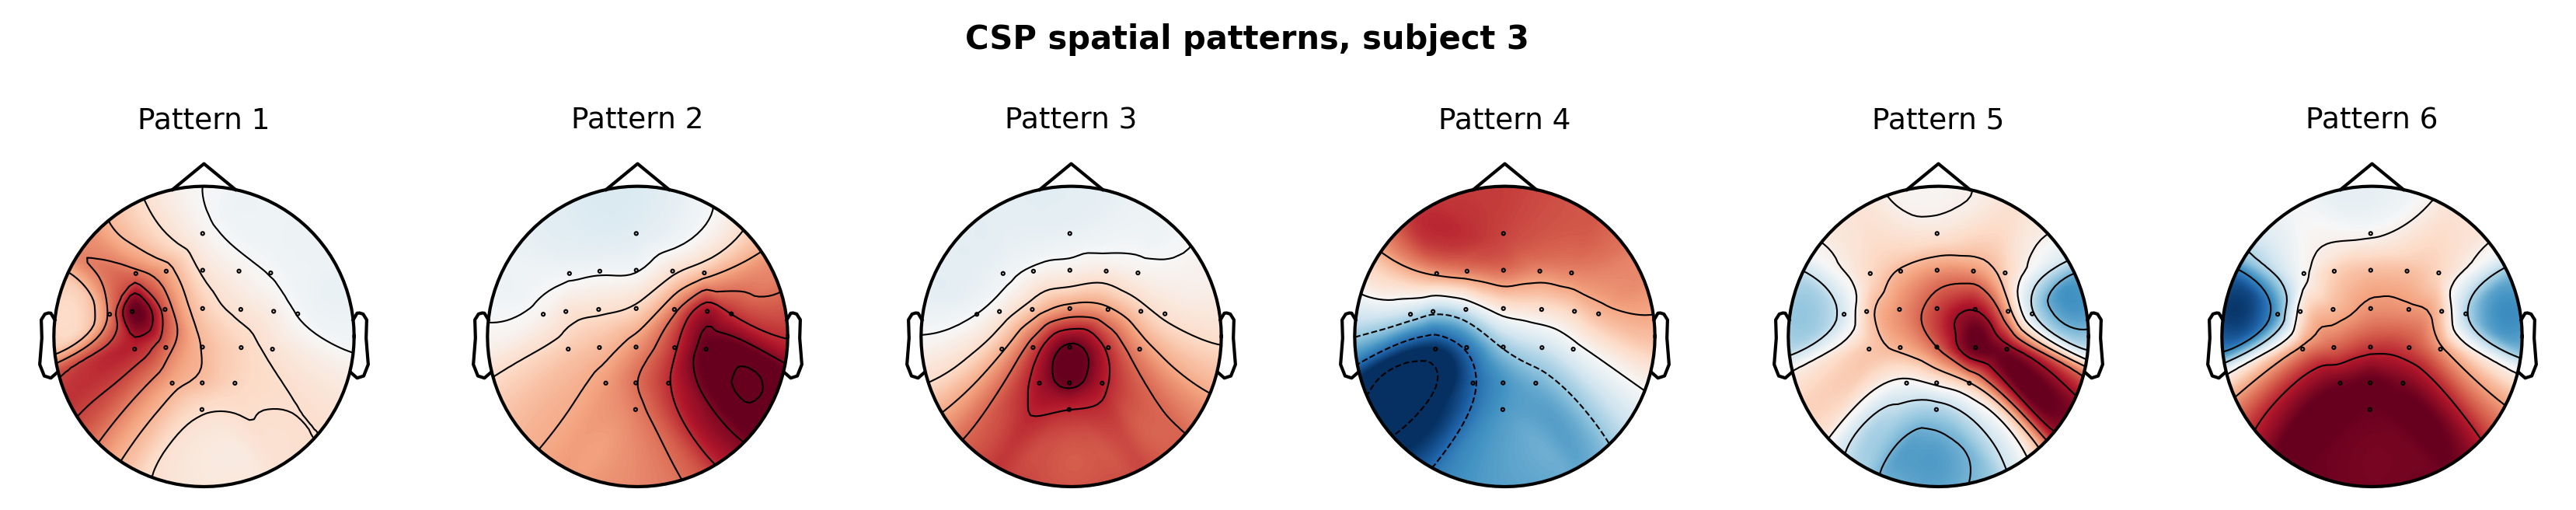
\includegraphics[width=0.92\textwidth]{figA1_csp_patterns.png}
\caption{The six CSP spatial patterns of subject 3's decoder.}
\label{fig:csp}
\end{figure}

\textbf{Latency.} Decision time varies hugely between subjects: only 2\%
of subject~3's trials are censored, but 99--100\% of those of subjects 4
and 9 (\code{fig4\_latency.png}). These latencies, the confusion matrices
and the confidences are saved trial by trial to
\code{results/part1/decoder\_traces.csv}, which is the input to Part~2.

% =====================================================================
\section{Part 2: the shared-control simulator}

Recorded EEG cannot react to the wheelchair, so Part~2 builds a closed
loop in which every piece is either measured from Part~1 or a standard
model (Figure~\ref{fig:block}). The simulation steps every
$\Delta t = 20$\,ms.

\begin{figure}[htbp]
\centering
\resizebox{0.92\textwidth}{!}{%
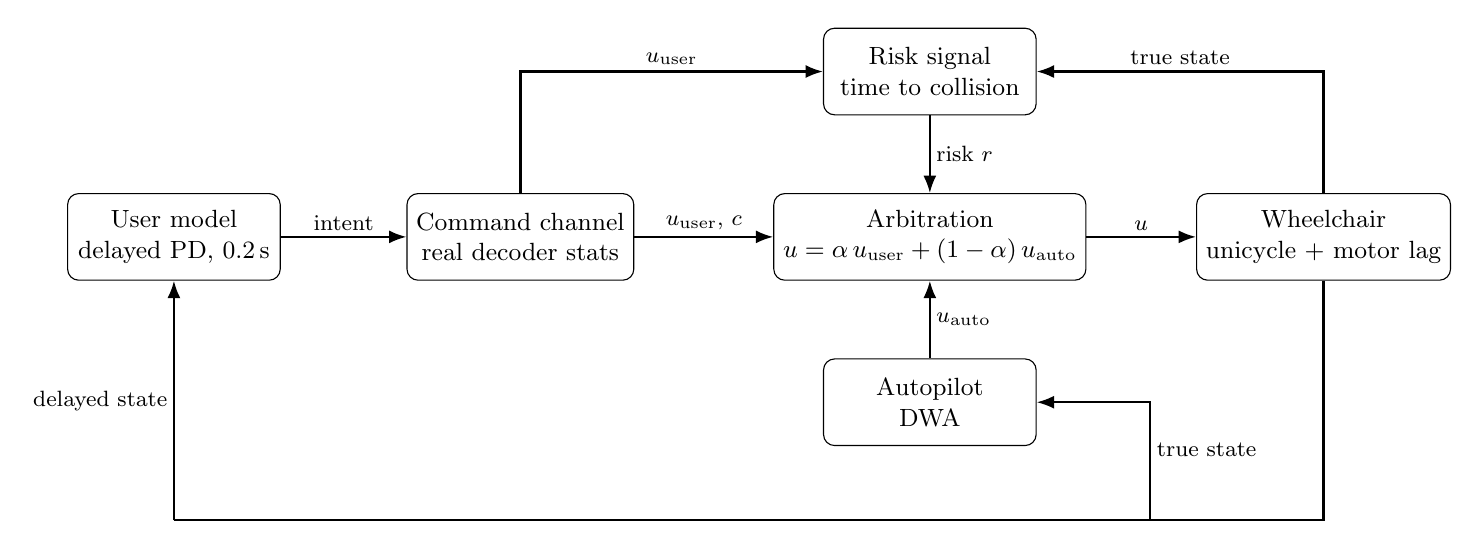
\begin{tikzpicture}[
   block/.style={draw, rounded corners, minimum width=2.7cm,
                 minimum height=1.1cm, align=center, font=\small},
   sig/.style={-{Latex[length=2.2mm]}, thick},
   lbl/.style={font=\footnotesize, inner sep=2pt}]
  \node[block] (op)    at (0,2)    {User model\\delayed PD, 0.2\,s};
  \node[block] (ch)    at (4.4,2)  {Command channel\\real decoder stats};
  \node[block, minimum width=3.6cm] (arb) at (9.6,2) {Arbitration\\$u=\alpha\,u_{\mathrm{user}}+(1-\alpha)\,u_{\mathrm{auto}}$};
  \node[block] (plant) at (14.6,2)  {Wheelchair\\unicycle + motor lag};
  \node[block] (risk)  at (9.6,4.1) {Risk signal\\time to collision};
  \node[block] (auto)  at (9.6,-0.1) {Autopilot\\DWA};
  % forward path
  \draw[sig] (op) -- node[lbl,above]{intent} (ch);
  \draw[sig] (ch) -- node[lbl,above]{$u_{\mathrm{user}}$, $c$} (arb);
  \draw[sig] (arb) -- node[lbl,above]{$u$} (plant);
  % risk and autopilot
  \draw[sig] (ch.north) |- node[lbl,above,pos=0.75]{$u_{\mathrm{user}}$} (risk.west);
  \draw[sig] (risk) -- node[lbl,right]{risk $r$} (arb);
  \draw[sig] (auto) -- node[lbl,right]{$u_{\mathrm{auto}}$} (arb);
  \draw[sig] (plant.north) |- node[lbl,above,pos=0.75]{true state} (risk.east);
  % feedback
  \draw[thick] (plant.south) |- (12.4,-1.6) -- (0,-1.6);
  \draw[sig] (0,-1.6) -- node[lbl,left]{delayed state} (op.south);
  \draw[sig] (12.4,-1.6) |- node[lbl,right,pos=0.3]{true state} (auto.east);
\end{tikzpicture}}
\caption{The closed loop. Only the user's path is delayed and corrupted;
the autopilot sees the true state. Risk is computed on the user's
command, because the question it answers is ``how bad would it be to
obey?''.}
\label{fig:block}
\end{figure}

\subsection{The command channel}
\label{sec:channel}
The channel reproduces the real decoder of one subject \ptwo{2}. At each
decision it does four things.

\textbf{1. Sample and hold.} Every 2\,s it takes one snapshot of the
user's intent and holds it until the next decision.

\textbf{2. Is the decision wrong? A two-state Markov chain.} Each
decision is either \emph{reliable} (right) or \emph{degraded} (wrong).
The chance of the next one being wrong may depend on the last one:
\begin{equation}
p_{rd} = P(\text{wrong now} \mid \text{right last time}),\qquad
p_{dd} = P(\text{wrong now} \mid \text{wrong last time}).
\end{equation}
If $p_{dd} > p_{rd}$, errors come in streaks; if $p_{dd} \approx p_{rd}$,
they are independent coin flips. The long-run error rate is
$\pi = p_{rd}/(p_{rd} + 1 - p_{dd})$, and the mean length of a run of
errors is $1/(1-p_{dd})$. Fitted to each subject's real sequence of right
and wrong decisions, a likelihood-ratio test finds significant streaks in
\textbf{0 of 9} subjects (mean streak 2.64 decisions, against 2.56 for
coin flips) \ptwo{2.2}. The reason is the class effect above: the cue
order is randomised, so the errors are too. We keep the chain and use
streakiness as a setting to sweep (Section~\ref{sec:ablations}).

\textbf{3. If wrong, which wrong command?} It is drawn from the
subject's confusion matrix with the correct answers removed
\ptwo{2.3}, and the user's intended direction is rotated by the angle
between the intended and the wrong command (Table~\ref{tab:mapping});
\emph{stop} sets the speed to zero.

\textbf{4. Delay and confidence.} The decision reaches the chair after a
latency drawn at random from that subject's measured latencies
(bootstrap) \ptwo{2.4}, and carries a confidence $c$ drawn from the
subject's real calibrated confidences, separately for right and wrong
decisions \ptwo{2.5}. Pooled over subjects, confidence separates right
from wrong decisions with an AUC of 0.676, but within one subject the gap
is only about 0.05: confidence is only weakly informative.

Together, the hold and the latency mean the command the chair acts on is
on average 2.95\,s old for subject~3 and 3.72\,s for subject~5
\ptwo{2.6}.

\subsection{The wheelchair model}
The wheelchair is a \emph{unicycle} \ptwo{3.1}: position $(x, y)$,
heading $\theta$, forward speed $v$ and turn rate $\omega$. It cannot
move sideways. Its motors respond with first-order lags:
\begin{equation}
\dot x = v\cos\theta,\qquad \dot y = v\sin\theta,\qquad \dot\theta = \omega,
\qquad
\dot v = \frac{v_{\mathrm{cmd}} - v}{\tau_v},\qquad
\dot\omega = \frac{\omega_{\mathrm{cmd}} - \omega}{\tau_\omega},
\label{eq:unicycle}
\end{equation}
with $\tau_v = 0.30$\,s and $\tau_\omega = 0.20$\,s, speed limits
$-0.4 \le v \le 1.2$\,m/s and $|\omega| \le 1.5$\,rad/s, and limits on
the accelerations. It drives in three rooms (Figure~\ref{fig:paths}
shows one): a 2\,m wide \emph{corridor}, a \emph{doorway} with a pillar
in the middle, and a \emph{cluttered} room \ptwo{3.3}.

\textbf{From intent to motor command.} The user and the channel speak in
\emph{intent vectors}, arrows meaning ``go that way, this hard''. If
$e_\theta$ is the angle between the arrow and the chair's heading,
\begin{equation}
\omega_{\mathrm{cmd}} = k\,e_\theta,\qquad
v_{\mathrm{cmd}} = \min\bigl(|\text{intent}|,\, v_{\max}\bigr)\,
\bigl(\max(\cos e_\theta,\, 0)\bigr)^{2},\qquad k = 2 .
\label{eq:intent}
\end{equation}
The squared-cosine factor makes a chair facing the wrong way stop and
turn instead of drifting.

\subsection{The user model}
The user is modelled as a PD controller that sees the chair 0.2\,s late
and always aims at the goal \ptwo{4}:
\begin{equation}
\text{intent}(t) = K_p\bigl(\text{goal} - p(t - \tau_h)\bigr) - K_d\,v(t - \tau_h),
\qquad K_p = 4,\; K_d = 2,\; \tau_h = 0.2\,\text{s}.
\label{eq:user}
\end{equation}
The P term pulls toward the goal, harder when far away; the D term
brakes against the speed already built up. The model \emph{does not
steer around obstacles}, which matters for every result below.

\subsection{The autopilot}
The autopilot uses the \emph{Dynamic Window Approach}
(DWA)~\cite{fox1997dwa}, a standard local planner for wheeled robots
\ptwo{5.2}. Several times a second it asks: of all the speeds and turn
rates the chair can actually reach in the next moment, given its motor
and acceleration limits (the ``dynamic window''), which one is best? It
predicts where each candidate would take the chair over the next 1.5\,s,
throws away any that would come too close to an obstacle, and among the
rest prefers the one that makes the most progress toward the goal while
keeping a safe distance and a reasonable speed. Progress is measured
along the shortest path to the goal \emph{around} the obstacles, not in a
straight line, so the autopilot does not get stuck in front of the
pillar.

DWA is a planner, not a linear controller, so it has no transfer
function. For the stability analysis (Section~\ref{sec:stability}) the
autopilot is therefore represented by a linear stand-in, an LQR
controller, whose gains are derived in \code{math\_derivation.pdf}.

\subsection{The risk signal}
Risk asks: \emph{if the chair obeyed the user's command, how soon would it
crash?} The \emph{time to collision} ($\TTC$) is found by following the
arc of the user's $(v, \omega)$ forward in 0.05\,s steps until it touches
an obstacle (at most 3\,s ahead). It is mapped to $[0, 1]$ and smoothed
with a 0.3\,s first-order lag \ptwo{5.3}:
\begin{equation}
r_{\mathrm{raw}} =
\begin{cases}
0, & \TTC \ge 3\,\text{s},\\[2pt]
\dfrac{3 - \TTC}{3 - 0.5}, & 0.5\,\text{s} < \TTC < 3\,\text{s},\\[8pt]
1, & \TTC \le 0.5\,\text{s},
\end{cases}
\qquad
r \leftarrow r + \bigl(1 - e^{-\Delta t/0.3}\bigr)\,(r_{\mathrm{raw}} - r).
\label{eq:risk}
\end{equation}

\subsection{Six ways to share control}
\label{sec:rules}
Every rule except the safety filter applies the blend \eqref{eq:blend} to
the chair's own inputs $u = (v_{\mathrm{cmd}}, \omega_{\mathrm{cmd}})$
\ptwo{5.4}:

\begin{table}[H]
\centering\small
\begin{tabular}{@{}llp{7.2cm}@{}}
\toprule
Rule & User's share $\alpha$ & Why it is in the comparison \\
\midrule
\code{manual\_only}     & 1                     & baseline: the user alone \\
\code{autonomy\_only}   & 0                     & baseline: the autopilot alone \\
\code{fixed\_blend}     & 0.5 (and a sweep 0--1) & the simplest sharing rule \\
\code{confidence\_only} & $c$                   & trust the user as much as the decoder trusts itself \\
\code{adaptive}         & $c\,(1-r)$, gated and smoothed & \textbf{the rule under study} \\
\code{safety\_filter}   & not a blend           & obey the user unless $\TTC < 1.5$\,s, then use the closest safe command \\
\bottomrule
\end{tabular}
\caption{The six sharing rules.}
\label{tab:rules}
\end{table}

\textbf{The adaptive rule, intuitively.} The rule starts from
$\alpha = c\,(1-r)$: the user gets a large share only when the decoder is
confident \emph{and} the path ahead is safe; if either is low, control
shifts to the autopilot. Two practical details are added on top. First,
control is handed back and forth with some reluctance: once the user's
share has been taken away, it is returned only after the situation has
clearly improved, so that control does not flicker between the two
drivers when the signals hover near a threshold. Second, $\alpha$ changes
smoothly and not too fast, because it multiplies a feedback path and a
sudden jump would jolt the chair. The exact thresholds and time constants
are in \ptwo{5.4}.

\textbf{The safety filter} passes the user's command through untouched
while $\TTC > 1.5$\,s. Below that, it picks the safe DWA candidate closest
to the user's command, measured as
$(\Delta v/v_{\max})^2 + (\Delta\omega/\omega_{\max})^2$.

\textbf{Why blending can fail} \ptwo{5.5}. Two commands can each be safe
while their average is not. In front of the pillar, ``turn left'' and
``turn right'' are both safe, but their 50/50 blend has zero turn rate
and full forward speed, so it drives straight into the pillar. This is a
property of a vehicle that cannot move sideways, and it is why the safety
filter, which never averages, is part of the comparison.

% =====================================================================
\section{Results}

\textbf{Experiment.} Each rule was run on 9 subjects $\times$ 3 rooms
$\times$ 20 random seeds = 540 drives. The random numbers of a drive
depend on (subject, room, seed) but not on the rule, so all six rules
meet exactly the same decoder errors, delays and confidences: the
comparison is \emph{paired} \ptwo{6.1}. A drive succeeds if the chair gets
within 0.35\,m of the goal, and fails on a collision or after 60\,s.
Including the parameter sweeps and ablations, 32,400 drives were run.

\subsection{Main comparison}

\begin{table}[H]
\centering\small
\begin{tabular}{@{}lrrrrrrrr@{}}
\toprule
 & \multicolumn{4}{c}{Success rate} & & & & \\
\cmidrule(lr){2-5}
Rule & all & corridor & doorway & cluttered & Crash & Time (s) & Mean $\alpha$ & Intervention \\
\midrule
\code{manual\_only}     & 0.119 & 0.333 & 0.022 & 0.000 & 0.881 & 9.3  & 1.000 & 0.000 \\
\code{autonomy\_only}   & 1.000 & 1.000 & 1.000 & 1.000 & 0.000 & 10.5 & 0.000 & 0.913 \\
\code{fixed\_blend}     & 0.161 & 0.400 & 0.083 & 0.000 & 0.839 & 9.8  & 0.500 & 0.933 \\
\code{confidence\_only} & 0.315 & 0.644 & 0.267 & 0.033 & 0.683 & 10.2 & 0.387 & 0.931 \\
\textbf{\code{adaptive}} & \textbf{0.996} & 1.000 & 1.000 & 0.989 & \textbf{0.004} & 11.7 & 0.118 & 0.914 \\
\code{safety\_filter}   & 0.356 & 0.689 & 0.356 & 0.022 & 0.120 & 44.8 & 0.771 & 0.350 \\
\bottomrule
\end{tabular}
\caption{Main comparison, 540 paired drives per rule; 180 per room
(\code{headline\_main.csv}, \code{success\_by\_room.csv}, \ptwo{6.7}).
Time is the mean length of a drive, until the goal, a crash or the 60\,s limit. Intervention is the share of time steps in
which the motors received something other than the user's command.}
\label{tab:headline}
\end{table}

\begin{itemize}\setlength{\itemsep}{2pt}
\item \textbf{The user alone} succeeds in 12\% of drives, and almost never
outside the corridor.
\item \textbf{Fixed blending} (16\%) and \textbf{confidence alone} (32\%)
help only a little.
\item \textbf{The safety filter} cuts crashes to 12\% but succeeds only
36\% of the time and takes 45\,s on average: it prevents crashes but does
not make progress, because by the time $\TTC$ drops below 1.5\,s the chair
is often already committed.
\item \textbf{Adaptive} reaches \textbf{99.6\%} success with 0.4\%
crashes while giving the user about 12\% of the control, close to the
autopilot's 100\%.
\end{itemize}

Not all of the user-alone failure is the decoder's fault. With a
\emph{perfect} decoder, the user alone still crashes in every doorway
and cluttered-room drive, because the user model aims straight through
obstacles. Only the corridor isolates the decoder's cost: 100\% success
with a perfect decoder, 33\% with the real one \ptwo{6.5}.

\begin{figure}[htbp]
\centering
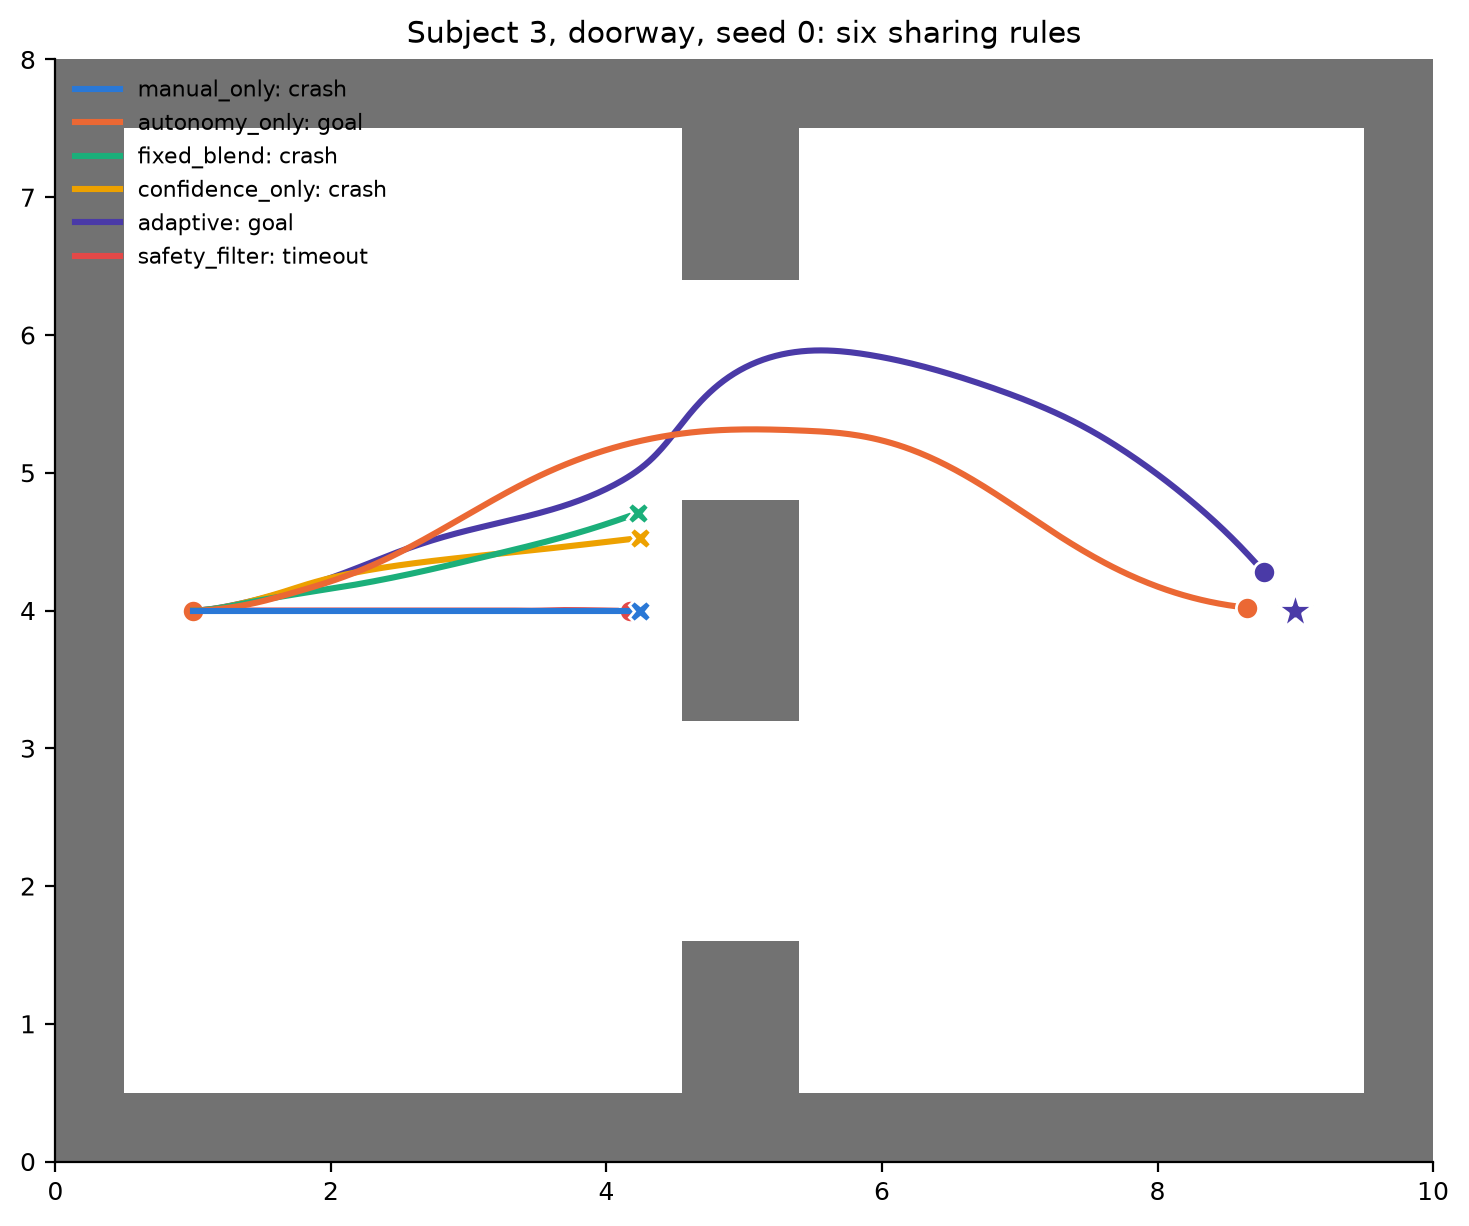
\includegraphics[width=0.78\textwidth]{12_s6_six_paths_doorway.png}
\caption{One doorway drive (subject 3, seed 0) under all six rules. Only
the autopilot and \code{adaptive} pass the pillar; the safety filter
stalls in front of it \ptwo{6.3}.}
\label{fig:paths}
\end{figure}

Figure~\ref{fig:trace} shows what \code{adaptive} does during that drive.
The user gets real control (up to $\alpha \approx 0.6$) when the decoder
is confident and the way is clear, and loses it as the chair approaches
the pillar. In this drive every decoded command was \emph{correct}: the
risk term is protecting against a correctly decoded but unsafe command,
which confidence could never catch.

\begin{figure}[htbp]
\centering
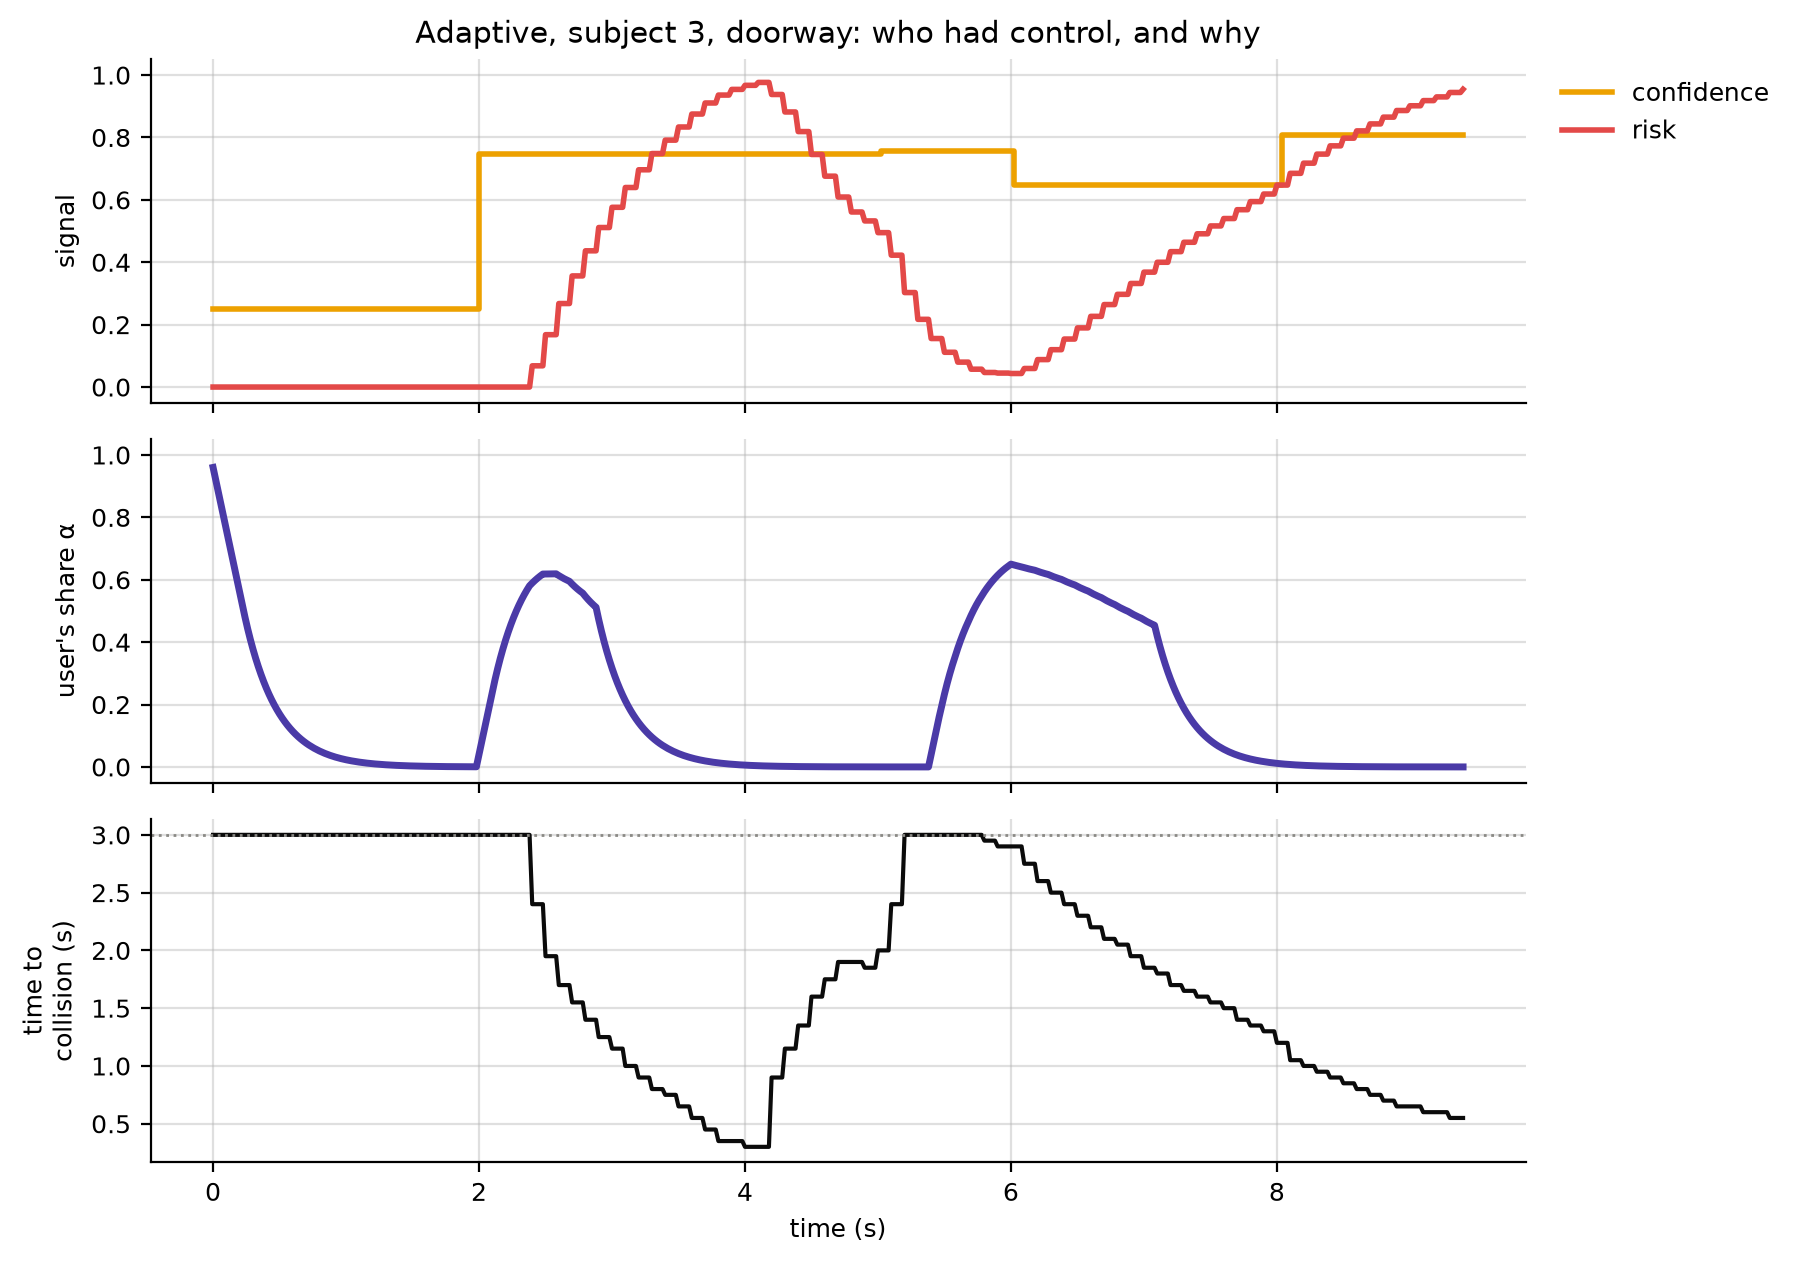
\includegraphics[width=0.55\textwidth]{13_s6_adaptive_trace.png}
\caption{Inside one \code{adaptive} drive: confidence and risk (top), the
user's share $\alpha$ (middle), and time to collision (bottom)
\ptwo{6.6}.}
\label{fig:trace}
\end{figure}

\subsection{Is adaptive really as good as the autopilot?}
The 540 drives per rule are not 540 independent samples: they come from
only 9 people, and drives of the same person are alike. Treating them as
independent would make every difference look significant. So for each
subject we average the paired difference in success over their 60 drives
and bootstrap a 95\% confidence interval over the 9 subjects \ptwo{6.8}.

\begin{table}[H]
\centering\small
\begin{tabular}{@{}lrc@{}}
\toprule
\code{adaptive} minus & Difference in success rate & 95\% CI (subject level) \\
\midrule
\code{manual\_only}     & $+0.878$ & $[+0.791,\ +0.957]$ \\
\code{fixed\_blend}     & $+0.835$ & $[+0.735,\ +0.924]$ \\
\code{confidence\_only} & $+0.681$ & $[+0.604,\ +0.757]$ \\
\code{safety\_filter}   & $+0.641$ & $[+0.576,\ +0.726]$ \\
\code{autonomy\_only}   & $-0.004$ & $[-0.009,\ \phantom{+}0.000]$ \\
\bottomrule
\end{tabular}
\caption{Paired differences in success rate at the subject level
(\code{paired\_subject\_level.csv}).}
\label{tab:paired}
\end{table}

Against four of the rules, \code{adaptive} is clearly better: it raises
the success rate by 0.64 to 0.88, and every interval excludes zero
(Table~\ref{tab:paired}). Against the autopilot, the interval
$[-0.009, 0.000]$ stays above $-0.02$, the non-inferiority margin, so
adaptive is \emph{non-inferior} (not meaningfully worse); but it is never
better, and 7 of the 9 subjects show exactly zero difference. The honest
claim is therefore: \emph{the user can be given some control back without
losing the autopilot's safety, as long as the sharing rule looks at
risk.} Whether that 12\% of control matters to a real user cannot be
measured in a simulation.

\subsection{Does a better decoder give a better wheelchair?}
For the fixed blend and the safety filter, yes: success rises with
decoder quality (Pearson $r = 0.55$ and $0.69$ across the 9 subjects).
Under \code{adaptive} the link is broken ($r = -0.125$, $p = 0.75$): every
subject reaches 0.98--1.00, including subject~5 whose decoder is below
chance (Figure~\ref{fig:kappa}, \code{success\_vs\_kappa.csv}).

\begin{figure}[htbp]
\centering
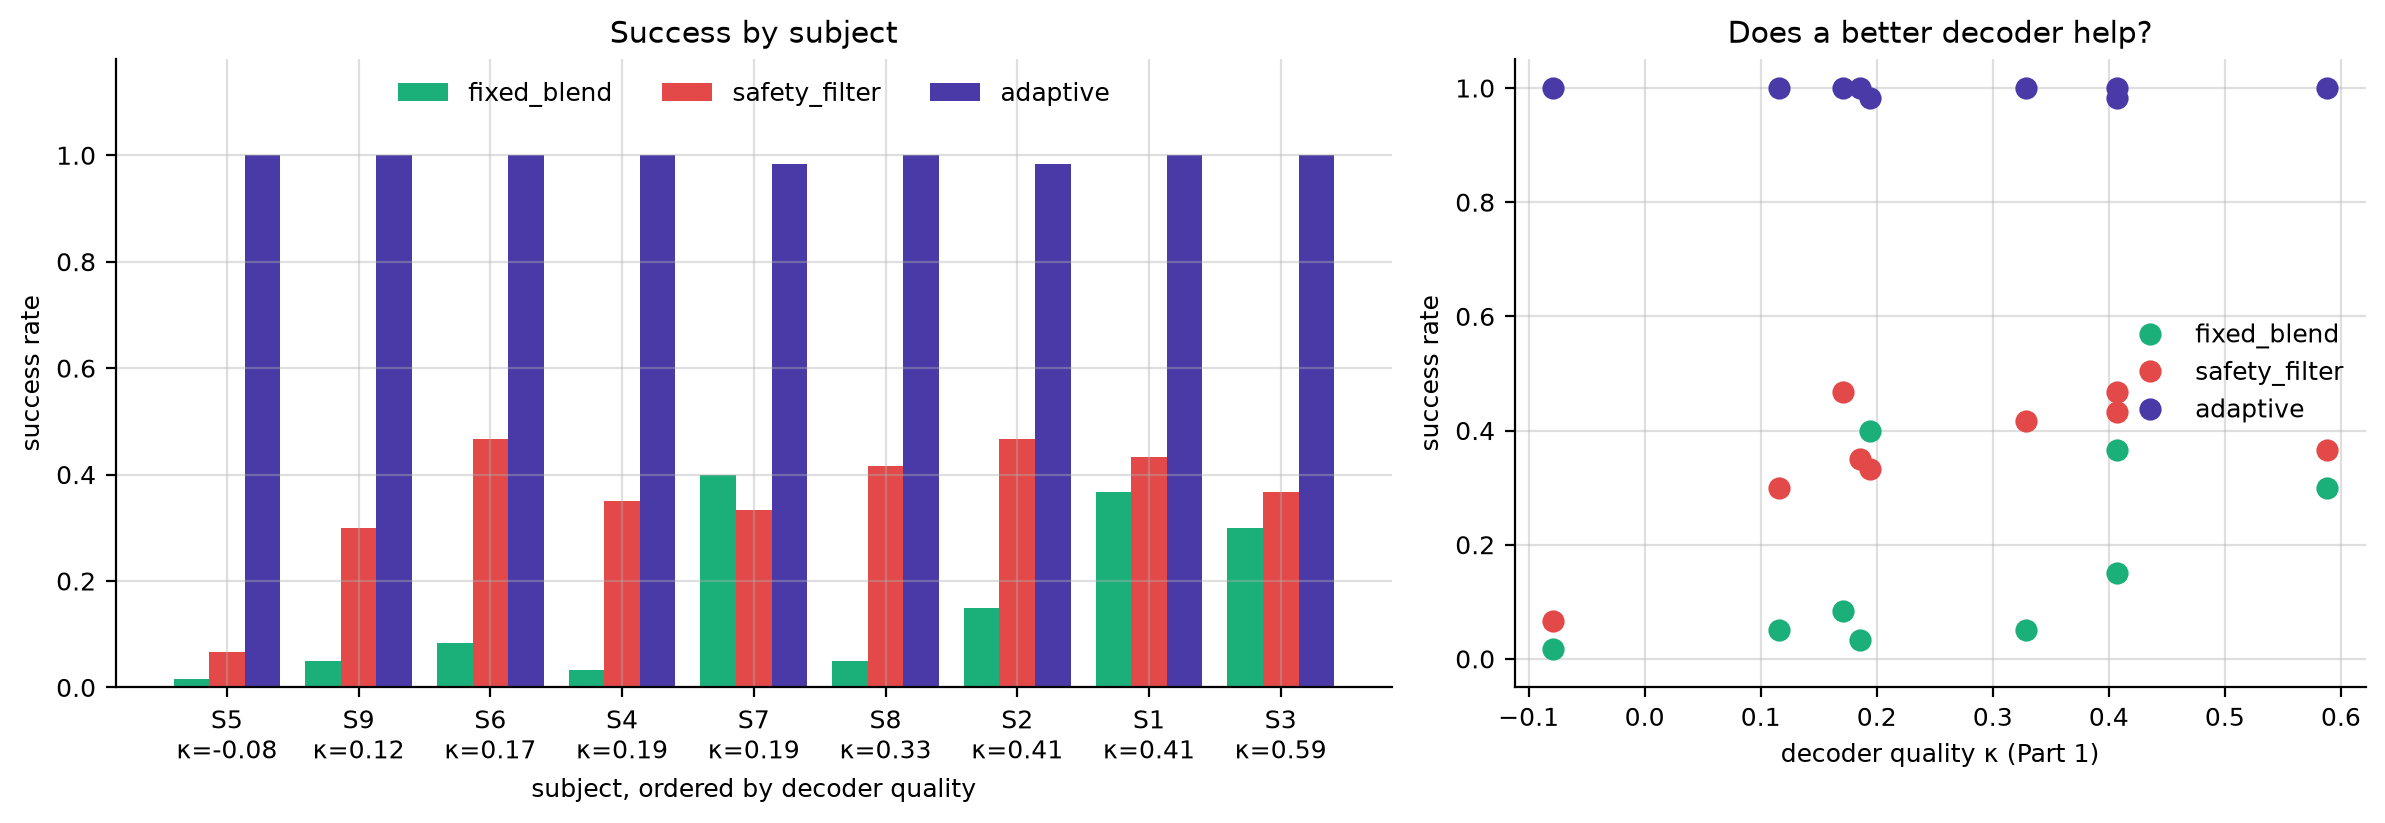
\includegraphics[width=0.82\textwidth]{14_s6_success_vs_kappa.png}
\caption{Success per subject, ordered by decoder quality $\kappa$ from
Part 1 \ptwo{6.9}.}
\label{fig:kappa}
\end{figure}

\subsection{How much fixed control is too much?}
With a \emph{fixed} share, the chair is safe only up to $\alpha = 0.1$;
crashes rise fastest around $\alpha = 0.2$ (Figure~\ref{fig:sweep}). A
fixed $\alpha = 0.1$ is therefore also 100\% safe and gives the user 10\%
of the control, close to adaptive's 12\% average. What adaptive changes
is the \emph{timing}: almost no control near obstacles, and 0.6 or more
when the way is clear.

\begin{figure}[htbp]
\centering
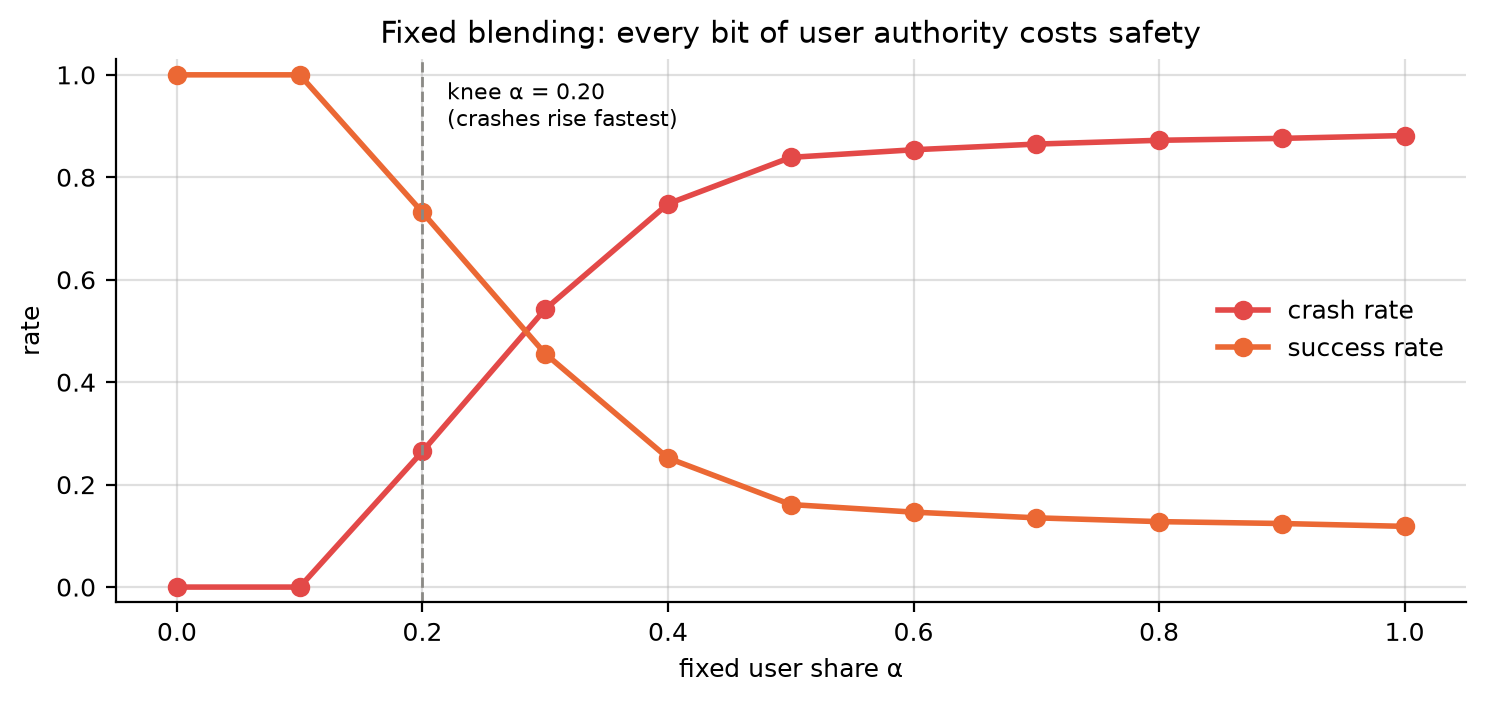
\includegraphics[width=0.6\textwidth]{15_s6_alpha_sweep.png}
\caption{Success and crash rate for a fixed user share
(\code{alpha\_sweep.csv}, \ptwo{6.10}).}
\label{fig:sweep}
\end{figure}

\subsection{Which part of the rule does the work?}
\label{sec:ablations}
An \emph{ablation} switches one piece off and re-runs every drive with the
same random numbers \ptwo{6.11}.

\begin{table}[H]
\centering\small
\begin{tabular}{@{}llrrr@{}}
\toprule
Ablation & What changes & \code{adaptive} & \code{safety\_filter} & \code{confidence\_only} \\
\midrule
baseline & --- & 0.996 & 0.356 & 0.315 \\
\code{no\_risk\_term} & risk forced to 0 & \textbf{0.796} & \textbf{0.119} & 0.315 \\
\code{perfect\_confidence} & oracle: 1 if right, 0 if wrong & 0.996 & 0.356 & 0.507 \\
\code{no\_delay} & user's 0.2\,s delay removed & 0.996 & 0.350 & 0.320 \\
\code{no\_burst\_errors} & errors as coin flips & 0.996 & 0.344 & 0.309 \\
\code{confidence\_decay} & confidence fades with age & 1.000 & 0.356 & 0.569 \\
\bottomrule
\end{tabular}
\caption{Success rate under each ablation (\code{ablations.csv}).}
\label{tab:ablations}
\end{table}

\begin{itemize}\setlength{\itemsep}{2pt}
\item \textbf{Risk does the work.} Removing it drops \code{adaptive} from
0.996 to 0.796 (and the safety filter, which also uses $\TTC$, from 0.356
to 0.119).
\item \textbf{Confidence barely matters.} Even a perfect confidence signal
changes nothing for \code{adaptive}. It does help \code{confidence\_only}
(+0.19), where confidence is all the rule has.
\item \textbf{Fading confidence helps for the wrong reason.} It mainly
\emph{lowers} $\alpha$, giving the user less control; that, not better
information, is why it helps \code{confidence\_only}.
\item \textbf{Delay and streaks do not matter here.} There are no streaks
to remove, and removing 0.2\,s from a loop whose commands are already
3--4\,s old changes little. Section~\ref{sec:stability} gives the deeper
reason.
\end{itemize}
Part of why risk wins is the user model: it often asks for commands that
are \emph{correctly decoded but unsafe}, which confidence cannot catch.

A separate sweep made errors 1.5, 2.5 and 4 times streakier than coin
flips while keeping each subject's error rate fixed. \code{adaptive}
stays at 0.994--0.998 (\code{burstiness.csv}, \ptwo{6.12}), but this is
not proof of robustness: an adaptive drive lasts only about 5 decoder
decisions, too short to contain a long streak.

% =====================================================================
\section{Stability under delay}
\label{sec:stability}

\textbf{Why delay matters.} A feedback controller acting on old
information overshoots, and with enough delay each overshoot is larger
than the last: the loop becomes unstable. In the shared loop only the
user's path is delayed, and $\alpha$ sets how much weight it gets. So we
ask: \emph{for each share $\alpha$, what is the largest loop delay
$\tau_{\max}(\alpha)$ before the loop becomes unstable?}

\textbf{Model.} The full wheelchair is nonlinear, so for an exact answer
we analyse one axis of a damped point mass, $\dot p = v$,
$\dot v = u - d\,v$ ($d = 1$), with the autopilot as an LQR controller
$\ua = -K_1 z - K_2\dot z$ (no delay) and the user as the delayed PD
controller \eqref{eq:user}, where $z = p - \text{goal}$. The closed loop
is a delay differential equation, and its characteristic equation is
\begin{equation}
\boxed{\;s^2 + d\,s + (1-\alpha)(K_1 + K_2 s) + \alpha\,(K_p + K_d s)\,e^{-\tau s} = 0\;}
\label{eq:char}
\end{equation}

\textbf{Derivation in brief.} The full step-by-step derivation, with the
reasoning behind each step, is in \code{math\_derivation.pdf}:
\begin{enumerate}\setlength{\itemsep}{1pt}
\item The LQR gains come from solving the Riccati equation by hand:
$K_1 = \sqrt{10} = 3.162278$, $K_2 = 1.885231$ (\S3 there).
\item Because of $e^{-\tau s}$, equation \eqref{eq:char} has infinitely
many roots, so Routh--Hurwitz and root locus cannot be used (\S4). The
loop is stable at $\tau = 0$, and it can only become unstable when a root
crosses the imaginary axis, at some $s = j\omega$.
\item At $s = j\omega$ the delay only rotates the user's term without
changing its size, so it drops out of the condition, leaving a quadratic
in $X = \omega^2$ (\S5):
\begin{equation}
X^2 + bX + c = 0,\qquad
b = P_2^2 - Q_2^2 - 2P_1,\qquad c = P_1^2 - Q_1^2,
\end{equation}
with $P_1 = (1-\alpha)K_1$, $P_2 = d + (1-\alpha)K_2$, $Q_1 = \alpha K_p$,
$Q_2 = \alpha K_d$.
\item Each positive root gives a crossing frequency $\omega_i$ and phase
$\theta_i$, hence a delay $\tau_i = \theta_i/\omega_i$, and
$\tau_{\max}(\alpha) = \min_i \tau_i$ (\S6). If there is no positive
root, the loop is stable for every delay (\S7), which happens for
$\alpha$ below about $K_1/(K_1 + K_p) = 0.4415$.
\end{enumerate}

\begin{figure}[htbp]
\centering
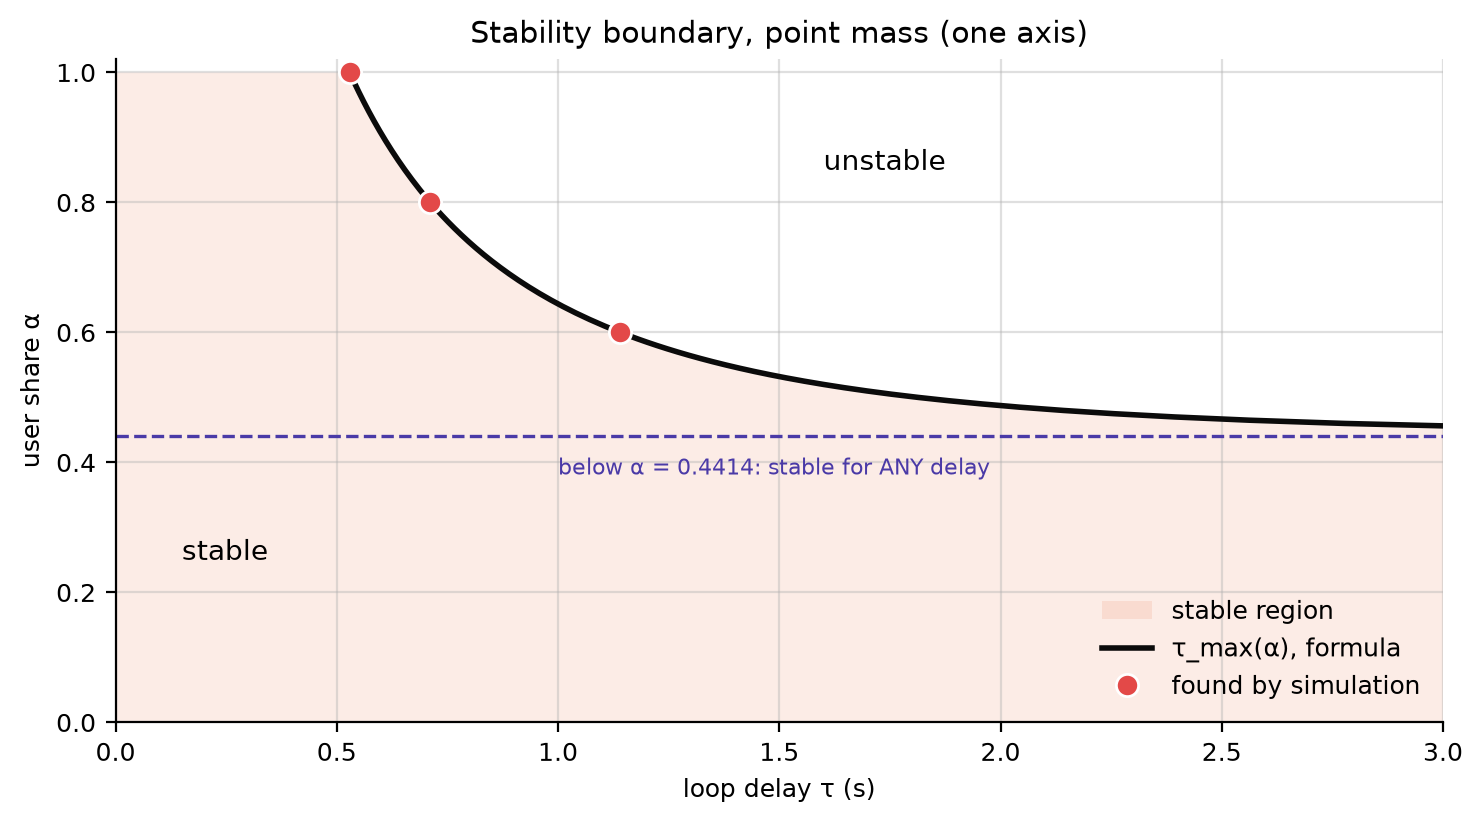
\includegraphics[width=0.62\textwidth]{17_s7_stability_boundary.png}
\caption{Stability boundary $\tau_{\max}(\alpha)$ for the point mass. The
curve is the exact formula; the dots are boundaries found by simulating
the delay equation directly, with no formula involved
(\code{tau\_max\_curve.csv}, \ptwo{7.1--7.2}).}
\label{fig:stab}
\end{figure}

\begin{table}[H]
\centering\small
\begin{tabular}{@{}ll@{}}
\toprule
Quantity & Value \\
\midrule
LQR gains $K_1$, $K_2$ & 3.162278, 1.885231 \\
User gains $K_p$, $K_d$; plant damping $d$ & 4, 2; 1 \\
$\tau_{\max}$ with the user alone ($\alpha = 1$) & \textbf{0.529\,s} \\
Stable for \emph{any} delay below & $\alpha = 0.4414$ \\
Simple bound $\alpha^* = K_1/(K_1+K_p)$ (slightly too high here) & 0.4415 \\
Formula vs.\ \code{control} library ($\alpha = 1$) & differ by $2.2\times10^{-16}$\,s \\
Formula vs.\ direct simulation ($\alpha = 0.6, 0.8, 1$) & relative error $\le 4\times10^{-6}$ \\
Pad\'e(2,2) over-estimate of $\tau_{\max}$ & 0.33\% ($\alpha=1$) to 2.55\% ($\alpha=0.5$) \\
Wheelchair heading loop: $\alpha^*$ (exact), $\tau_{\max}(1)$ & 0.6126, 0.647\,s \\
\bottomrule
\end{tabular}
\caption{Stability results (\code{logs/part2\_run.log},
\code{pade\_vs\_exact.csv}, \code{tau\_max\_formula\_vs\_simulation.csv}).}
\label{tab:stab}
\end{table}

\textbf{Reading the result.} The more weight the delayed user gets, the
less delay the loop tolerates. Below $\alpha \approx 0.44$ the undelayed
autopilot is strong enough to hold the loop whatever the delay. At
$\alpha = 1$, $\tau_{\max}$ equals the classical delay margin (phase
margin divided by crossover frequency). The common Pad\'e shortcut always
\emph{over-estimates} the margin, the unsafe direction, which is why we use
the exact solution.

\textbf{Does this boundary limit the simulated wheelchair? No}
\ptwo{7.5}. The user-alone chair runs with commands 3--4\,s old, well past
its heading loop's 0.647\,s margin, yet it does not oscillate. The reason
is structural: in the simulator the user's \emph{target} is delayed, but
the chair's own heading feedback is not, and a delayed reference cannot
destabilise a stable loop. Moreover, \code{adaptive} spends most of its
time below the heading loop's $\alpha^* = 0.6126$, where no delay can
cause instability (92\% of the steps in the drive of
Figure~\ref{fig:trace}). Together with the ablations, this points to one
conclusion: \textbf{this system is limited by decoder error, not decoder
latency.}

% =====================================================================
\section{Challenges}
A few problems took most of the effort; each changed the final design.
\begin{itemize}\setlength{\itemsep}{2pt}
\item \textbf{The delay analysis.} The characteristic equation with
$e^{-\tau s}$ is not a polynomial, so the tools from the course
(Routh--Hurwitz, root locus) do not apply directly, and the Pad\'e
approximation turned out to over-estimate the margin. Finding an exact
method, and checking it against direct simulation, took several
attempts.
\item \textbf{Getting a fair simulation from offline EEG.} Recorded EEG
cannot react to the wheelchair, so the decoder had to be replaced by a
model built from its measured behaviour, and the human by a user model.
\item \textbf{The autopilot stuck at the pillar.} Scoring progress by the
straight-line direction to the goal left the autopilot undecided in front
of the symmetric pillar (0\% success); a navigation field fixed it.
\item \textbf{Blending two safe commands can be unsafe}, which led to
including a rule that never averages.
\item \textbf{Honest statistics.} With only 9 subjects, the drives are not
independent; the comparisons are therefore paired and the confidence
intervals computed at the subject level.
\end{itemize}

% =====================================================================
\section{Limitations}
\begin{itemize}\setlength{\itemsep}{2pt}
\item \textbf{The user is a model.} It always knows the goal, never
adapts, and does not avoid obstacles. This is the largest gap, and it
favours risk over confidence.
\item \textbf{User agency is not measured.} The case for \code{adaptive}
over the autopilot is that it gives control back; nothing here shows
that this matters to a person.
\item \textbf{Offline EEG.} The decoder enters through a model fitted to
recorded data, not as a live closed-loop signal, and a cued, randomised
experiment may hide error streaks that a self-paced BCI would show.
\item \textbf{Simple world.} Three hand-built 2-D rooms, static obstacles,
a perfect map and exact position.
\item \textbf{Stability is for a frozen $\alpha$}, a constant delay and a
linear model; \code{adaptive} varies $\alpha$ (slowly, by design), so the
boundary is a guide, not a proof for the full system.
\end{itemize}

% =====================================================================
\section{Conclusion and future work}
A motor-imagery decoder that is right 44\% of the time cannot drive a
wheelchair on its own: the user alone reaches the goal in 12\% of drives.
Sharing control with an autopilot fixes this, but \emph{how} the share is
chosen matters. A fixed share is safe only if the user gets almost
nothing ($\alpha \le 0.1$), and averaging two safe commands can be
unsafe. Gating the user's share on \emph{situational risk},
$\alpha = c\,(1-r)$, reaches 99.6\% success, keeps every subject at 0.98
or above, and breaks the link between decoder quality and task success;
the decoder's confidence adds almost nothing on top. On the theory side,
the delay boundary of the shared loop has an exact solution, verified by
simulation, but it is not what limits this system: the limit is the
decoder's errors.

\textbf{Future work.}
\begin{itemize}\setlength{\itemsep}{2pt}
\item Write up the results as a research paper and submit it for
publication.
\item Replace the recorded data with a real BCI headset, first in
simulation with live EEG and then, if given the chance, in practical
trials with users steering a real or scaled wheelchair.
\item An obstacle-aware, adapting user model, and a self-paced (uncued)
BCI where errors may really come in streaks.
\item Extend the stability analysis to a time-varying share $\alpha(t)$,
the 2\,s sample-and-hold, and the full wheelchair model
(see \code{math\_derivation.pdf}, \S10).
\end{itemize}

\textbf{Reproducing.} \code{README.md} gives the exact steps: install the
packages in \code{requirements.txt}, run the Part~1 notebook, then the
Part~2 notebook. Part~2 re-simulates 72 drives and checks them against the
saved log \code{results/part2/episodes.csv}: all 72 give the same outcome,
and every metric agrees to about one part in $10^{9}$ \ptwo{6.4}.

% =====================================================================
\begin{thebibliography}{10}\small
\setlength{\itemsep}{1pt}

\bibitem{brunner2008graz}
C.~Brunner, R.~Leeb, G.~R. M\"uller-Putz, A.~Schl\"ogl, and G.~Pfurtscheller.
BCI Competition 2008 -- Graz data set A. Graz University of Technology,
2008. \url{https://www.bbci.de/competition/iv/desc_2a.pdf}

\bibitem{tangermann2012review}
M.~Tangermann et al.
Review of the BCI Competition IV.
\emph{Frontiers in Neuroscience}, 6:55, 2012.

\bibitem{jayaram2018moabb}
V.~Jayaram and A.~Barachant.
MOABB: Trustworthy algorithm benchmarking for BCIs.
\emph{Journal of Neural Engineering}, 15(6):066011, 2018.

\bibitem{ramoser2000csp}
H.~Ramoser, J.~M\"uller-Gerking, and G.~Pfurtscheller.
Optimal spatial filtering of single trial EEG during imagined hand movement.
\emph{IEEE Trans.\ Rehabilitation Engineering}, 8(4):441--446, 2000.

\bibitem{blankertz2011shrinkage}
B.~Blankertz, S.~Lemm, M.~Treder, S.~Haufe, and K.-R. M\"uller.
Single-trial analysis and classification of ERP components -- a tutorial.
\emph{NeuroImage}, 56(2):814--825, 2011.

\bibitem{platt1999sigmoid}
J.~C. Platt.
Probabilistic outputs for support vector machines and comparisons to
regularized likelihood methods.
In \emph{Advances in Large Margin Classifiers}, pp.\ 61--74. MIT Press, 1999.

\bibitem{fox1997dwa}
D.~Fox, W.~Burgard, and S.~Thrun.
The dynamic window approach to collision avoidance.
\emph{IEEE Robotics \& Automation Magazine}, 4(1):23--33, 1997.

\bibitem{dragan2013blending}
A.~D. Dragan and S.~S. Srinivasa.
A policy-blending formalism for shared control.
\emph{Int.\ Journal of Robotics Research}, 32(7):790--805, 2013.

\bibitem{carlson2013wheelchairs}
T.~Carlson and J.~del~R. Mill\'an.
Brain-controlled wheelchairs: A robotic architecture.
\emph{IEEE Robotics \& Automation Magazine}, 20(1):65--73, 2013.

\end{thebibliography}

\end{document}
